% This is samplepaper.tex, a sample chapter demonstrating the
% LLNCS macro package for Springer Computer Science proceedings;
% Version 2.20 of 2017/10/04
%
\documentclass[runningheads]{llncs}
%
\usepackage{graphicx}
\usepackage[utf8]{inputenc}
% *** MATH PACKAGES ***
%
\usepackage{amsmath}
\usepackage{listings}% use mathematical symbols in Verbatim environment
\lstset{
  basicstyle=\ttfamily,
  mathescape
}
\usepackage{amsfonts,amssymb}
%\usepackage[linesnumbered,ruled,vlined]{algorithm2e}
\usepackage[linesnumbered,boxed,vlined]{algorithm2e}
% *** ALIGNMENT PACKAGES ***
%
\usepackage{array}
% *** PDF, URL AND HYPERLINK PACKAGES ***
%
\usepackage{url}



%personal defined packages
\usepackage{multirow,array}
% *** TABLE FOOTNOTE PACKAGES ***
\usepackage[bottom]{footmisc}
\usepackage{footnote}
\makeatletter
\def\@xfootnote[#1]{%
  \protected@xdef\@thefnmark{#1}%
  \@footnotemark\@footnotetext}
\makeatother
\usepackage{threeparttable}

\usepackage{caption}
\usepackage{subcaption}
\captionsetup{compatibility=false}

\usepackage{placeins}

 %table dash line
\usepackage{arydshln}

\usepackage{morefloats}

\begin{document}
%
\title{FPGA Key Generation Architectures for Post-Quantum Key Encapsulation Based on Quasi-Cyclic Codes}
%
%\titlerunning{Abbreviated paper title}
% If the paper title is too long for the running head, you can set
% an abbreviated paper title here
%
\author{Jingwei Hu\inst{1} \and Wen Wang\inst{2} \and Ray Cheung\inst{3} \and San Ling\inst{1} \and Huaxiong Wang\inst{1}}



\authorrunning{Jingwei Hu \textit{et. al.}}
% First names are abbreviated in the running head.
% If there are more than two authors, 'et al.' is used.
%


\institute{School of Physical and Mathematical Sciences, Nanyang Technological University, Singapore, \email{\{davidhu, HXWang, lingsan\}@ntu.edu.sg}
\and Department of Electrical Engineering, Yale University, USA,\\ \email{wen.wang.ww349@yale.edu}
\and Department of Electronic Engineering, City University of Hong Kong, Hong Kong, \email{r.cheung@cityu.edu.hk} }
%
\maketitle              % typeset the header of the contribution
%


\begin{abstract}
  In this paper, we present a fast and lightweight FPGA-based key generator for the
quantum-safe key encapsulation mechanism based on MDPC codes called BIKE which is among round-2 candidates for the NIST post-quantum standardization project. Existing hardware implementations
focus on the encryption/decryption or key encapsulation/decapsulation feature while few of them take into account
performance efficiency for the key generation which is particularly crucial for
KEM-based applications. The solution proposed here
aims at maximizing the metric of timing efficiency under a given resource restriction. New
parallelized polynomial multiplication algorithms are proposed to achieve this goal.
We show for instance that our highly optimized implementations for 128-bit security require $9.5\times 10^5$ cycles (0.597 ms), $2.1\times 10^6$ cycles (14.334 ms) and $9.8\times 10^5$ cycles (0.492 ms) to generate a key pair for BIKE-1/2/3. The proposed key generator is also area-efficient, uses only $544/1272/423$ slices for BIKE-1/2/3 on a small-size low-end Xilinx Spartan-7 FPGA.

\keywords{Post-Quantum Cryptography, Key Encapsulation Mechanism, Key Generator, QC-MDPC Code, FPGA Implementation}
\end{abstract}
%
%
%
\section*{Introduction}
Key encapsulation mechanisms (KEMs) are a class of encryption techniques designed to secure symmetric cryptographic key material for transmission using asymmetric (public-key) algorithms. Efficient and robust quantum-safe KEM design is a crucial and urgent topic in the cryptographic community. Recent years witnessed the NIST call for efficient and secure post-quantum KEMs in the post-quantum cryptography standardization competition \cite{chen2016report}.
The construction of a commercial quantum computer in not-so-distant future is a desperate threat to quantum-vulnerable primitives which are still relying on the hardness of the integer factorization problem or discrete logarithm problems such as the Diffie-Hellman key exchange, the Rivest-Shamir-Adleman (RSA) and Elliptic Curve Cryptography. Shor's algorithm \cite{shor1997polynomial} can be deployed on a quantum computer to solve both the integer factorization problem and the discrete logarithm problem in polynomial time. Code-based cryptosystems, which build their security on the hardness of decoding general linear codes, are among the most promising quantum-resisting candidates for which no known polynomial time attack on a quantum computer exists.

McEliece proposed the first code-based cryptosystem in 1978 \cite{mceliece1978public}, which uses  Goppa codes \cite{goppa1970new} as the underlying coding system. Goppa code-based schemes yield large public keys which limit the deployment of such systems in resource-constrained scenarios. Niederreiter proposed in 1986 another code-based system \cite{niederreiter1986knapsack} which exploits the same trapdoor, but uses the syndromes and parity-check matrices to construct the ciphertext and the key. It has been proved that Niederreiter and McEliece are equivalent \cite{li1994equivalence} and achieve the same security levels if the same family of codes is used.

Active research is focused on replacing Goppa codes with other families of structured codes that might lead to key size reduction. Nevertheless, this attempt may also compromise the system security. For example, some McEliece variants based on low-density parity-check (LDPC) codes \cite{monico2000using}, quasi-cyclic low-density parity-check (QC-LDPC) codes \cite{otmani2010cryptanalysis}, quasi-dyadic (QD) codes \cite{misoczki2009compact}, convolutional codes \cite{londahl2012new}, generalized Reed-Solomon (GRS) codes \cite{baldi2016enhanced}, and rank-metric codes \cite{loidreau2017new,gaborit2018polynomial} have been successfully attacked. Nevertheless, some variants exploiting the quasi-cyclic form  \cite{baldi2013optimization,baldi2008new,misoczki2013mdpc} have been shown to counteract the currently existing cryptanalysis attacks while achieving small-sized keys. A variety of KEMs built on the Niederreiter cryptosystem and LDPC/MDPC codes such as LEDAkem \cite{baldi2018ledakem}, CAKE \cite{barreto2017cake}, BIKE \cite{aragon2017bike}, also start to appear in the literature. BIKE and LEDAkem are currently on the round-2 candidate list for the post-quantum cryptography standardization. Recently, a new statistical attack, called reaction attack \cite{fabvsivc2017reaction,guo2016key} has been devised to recover the key by exploiting the information leaked from decoding failures in QC-LDPC and QC-MDPC code-based systems. The reaction attack is further enhanced in \cite{nilsson2019error} where the error pattern chaining method is introduced to generate multiple undecodable error patterns from an initial error pattern, thus improving the performance of such reaction attack in the CPA case. Nevertheless, the reaction attack only works for CPA systems and long-term keys, therefore, the deployment of a CCA2-secure conversion or ephemeral keys can resist the attack.


\textit{Related work.} Cryptographic hardware for the classical McEliece/Niederreiter schemes based on Goppa
codes has been extensively studied in the last decade. In 2009, the first FPGA-based implementation of McEliece's cryptosystem was proposed targeting
a Xilinx Spartan-3 FPGA and encrypted and decrypted data in 1.07 ms and 2.88 ms, using
security parameters achieving equivalence of 80-bit symmetric security~\cite{eisenbarth2009microeliece}.
The authors of~\cite{shoufan2010novel} presented another accelerator for McEliece encryption with binary Goppa codes on a more powerful Virtex5-LX110T, which is capable to encrypt and decrypt a message in 0.5 ms and 1.3 ms providing a similar level of security, respectively. Another publication~\cite{ghosh2012speed} based on
hardware/software co-design on a Spartan3-1400AN decrypts a message in 1 ms at 92 MHz with
the same level of security. Heyse and G\"uneysu in~\cite{heyse2012towards} report that a Goppa code-based Niederreiter decryption operation consumes 58.78 $\mu$s on a Virtex6-LX240T FPGA for $n = 2048$ and $t = 27$ for 80-bit symmetric security.  Wen Wang \textit{et.al.} present an FPGA-based key generator for the Goppa code-based Niederreiter cryptosystem \cite{wang2017fpga} and later a full implementation \cite{wang2018fpga} which includes modules for encryption, decryption, and key generation. Their designs generate a key pair in $3.98 ms$ for 256-bit security on a Xilinx Ultrascale+ FPGA.

The first implementation of MDPC code-based McEliece cryptosystem on embedded devices was presented in \cite{heyse2013smaller} in 2013. For 80-bit security, it is reported to run decryption in 125 $\mu$s with over 10,000 slices on Xilinx Virtex-6. A lightweight MDPC-McEliece has been implemented on FPGAs by sequentially manipulating cyclic rotations of the private key in block RAMs~\cite{von2014lightweight}. This lightweight design achieves circuit compactness which costs 64 slices for encryption and 148 slices for decryption on low-end Xilinx Spartan-6 device. An area-time efficient MDPC-Niederreiter has been implemented on FPGAs, which exploits a resource balanced MDPC decoding unit~\cite{hu2017area}. Their experimental results show the new architecture decrypts a message in 65 $\mu$s by using about 8,000 slices on a Virtex-6 FPGA.

\textit{Contributions.} Current progress focuses on key encapsulation/decpasulation. However, it should be considered to have a closer look at the
key generation as well. KEMs are used for ephemeral
key encapsulation and not for public-key encryption. Therefore, the key
generation is used as often as the encapsulation and decapsulation, \textit{i.e.},
we do have a strong motivation to accelerate the key generation since KEMs use ephemeral keys which require updating keys frequently.
As a consequence, this paper studies for the first time-efficient and compact FPGA-based key generation for a promising post-quantum KEM using MDPC codes (BIKE). The contributions include:
\begin{itemize}
  \item a fast and lightweight hardware architecture of BIKE for all secure parameters from 128-bit to 256-bit security.
  \item The timing scores ($9.55 \times 10^4$, $2.15 \times 10^6$, and $9.85 \times 10^4$ clock cycles for BIKE-1, BIKE-2, and BIKE-3, respectively) of our design outperform other embedded hardware and even powerful CPU with the dedicate carry-less multiplication instruction in terms of cycle counts.
  \item new polynomial multiplication algorithms (sparse-times-dense multiplication and generic algorithm) over ring $\mathbb{F}_2[x]/\langle x^r+1\rangle$ optimize the timing performance of key generation.
  \item constant time executions for all critical operations protect the proposed design from potential timing attacks.
\end{itemize}

\textit{Outline.} The paper is organized as follows. In Section 2, we describe BIKE. In Section~3, we present our design methodologies for implementing BIKE on reconfigurable devices. In particular, our new approaches for poynomial multiplication and squaring are detailed. In Section 4, a generic lightweight architecture for BIKE hardware is presented and discussed. In Section 5, experimental results on Xilinx FPGAs are shown to demonstrate the efficiency of the proposed techniques and hardware. In Section 6, some conclusions are drawn.

\section{Preliminaries for BIKE/LEDAkem Key Generation}

\newcommand{\tabincell}[2]{\begin{tabular}{@{}#1@{}}#2\end{tabular}}
%\begin{table*}[!t]\centering
%\caption{Parameters for LEDAkem according to NIST defined security category, referenced from \cite{baldi2018ledakem}}
%\label{table:systempar}
%\begin{minipage}{\textwidth}\centering
%\begin{tabular}{cc|cccccc}
%\hline
%\tabincell{c}{\textbf{Category}} &  $\mathbf{n_0}$ & $\mathbf{r}$ & $\mathbf{w}$ & \textbf{[$m_0,\cdots,m_{n_0-1}$]} & \textbf{t} & \textbf{SL} & \textbf{DFR}\\
%\hline
%\multirow{ 3}{*}{1} & 2 & 15,013 & 9 & [5,4] & 143 & \multirow{ 3}{*}{128} & $\leq 10^{-9}$\\
%                    & 3 & 9,643 & 13 & [3,2,2]&90 &                       & $\approx 10^{-9}$\\
%                    & 4 & 8,467 & 11 & [3,2,2,2]&72 &                     & $\approx 10^{-9}$\\
%\hline
%\multirow{ 3}{*}{2-3} & 2 & 24,533 & 13 & [5,4] & 208 & \multirow{ 3}{*}{192} & $\leq 10^{-8}$\\
%                      & 3 & 17,827 & 15 & [4,3,2]&129 &                       & $\leq 10^{-8}$\\
%                      & 4 & 14,717 & 15 & [3,2,2,2]&104 &                     & $\leq 10^{-8}$\\
%\hline
%\multirow{ 3}{*}{4-5} & 2 & 37,619 & 11 & [7,6] & 272 & \multirow{ 3}{*}{256} & $\leq 10^{-8}$\\
%                      & 3 & 28,477 & 13 & [5,4,4]&172 &                       & $\leq 10^{-8}$\\
%                      & 4 & 22,853 & 13 & [4,3,3,3]&135 &                     & $\leq 10^{-8}$\\
%\hline
%\end{tabular}
%\end{minipage}
%\end{table*}

\begin{table*}[!t]\centering
\caption{Parameters for BIKE according to NIST defined security category, referenced from \cite{aragon2017bike}}
\label{table:systempar}
\begin{minipage}{\textwidth}\centering
\begin{tabular}{cc|cccccc}
\hline
\tabincell{c}{\textbf{Category}} &  & $\mathbf{n}$ & $\mathbf{r}$ & $\mathbf{w}$ & \textbf{t} & \textbf{SL} & \textbf{DFR}\\
\hline
\multirow{ 2}{*}{1} & BIKE-[1,2] & 20,326 & 10,163 & 142 & 134 & \multirow{ 2}{*}{128} & \multirow{ 2}{*}{$\leq 10^{-7}$}\\
                    & BIKE-3 & 22,054 & 11,027 & 134 & 154 &                       & \\
\hline
\multirow{ 2}{*}{2-3} & BIKE-[1,2] & 39,706 & 19,853 & 206 &199 & \multirow{ 2}{*}{192} & \multirow{ 2}{*}{$\leq 10^{-7}$}\\
                      & BIKE-3 & 43,366 & 21,683 & 198 &226 &                       & \\
\hline
\multirow{ 2}{*}{4-5} & BIKE-[1,2] & 65,498 & 32,749 & 274 & 264 & \multirow{ 2}{*}{256} & \multirow{ 2}{*}{$\leq 10^{-7}$}\\
                      & BIKE-3 & 72,262 & 36,131 & 266 &300 &                       & \\
\hline
\end{tabular}
\end{minipage}
\end{table*}

\subsection{General Definitions}
\begin{table}[!tbh]
  \centering
  \begin{tabular}{ll}
     \hline
     % after \\: \hline or \cline{col1-col2} \cline{col3-col4} ...
     Polynomial View: &\\
     $\mathbb{F}_2$ & Finite field of 2 elements \\
     $\mathcal{R}$ & The cyclic polynomial ring $\mathbb{F}_2[x]/\langle x^r+1\rangle$\\
     $|x|$ & The Hamming weight of a binary polynomial $x$ \\
     $u \overset{\underset{\$}{}}{\gets} U$ & Variable $u$ is sampled uniformly at random from set $U$ \\
     \hline
     Matrix View: &\\
     $\mathcal{V}$ & The vector space of dimension $n$ over $\mathbb{F}_2$\\
     $\mathbf{m}$ & The vector over $\mathbb{F}_2$\\
     $\mathbf{G}$ & The matrix over $\mathbb{F}_2$\\
     \hline
   \end{tabular}
  \caption{Notations}\label{table:notation}
\end{table}

\begin{definition}{(Circulant Matrix)}
Let $\mathbf{x}=(x_0,\ldots,x_{n-1})\in \mathbb{F}^n$. The circulant matrix induced by $\mathbf{x}$ is defined and denoted as follows:
\[
 \mathbf{rot(x)} = \left[ \begin{array}{cccc}
        x_0 & x_{n-1} & \cdots &x_{1}\\
        x_{1} & x_{0} & \cdots &x_{2}\\
        \vdots & \vdots & \ddots & \vdots \\
        x_{n-1} & x_{n-2} & \cdots & x_{0}
        \end{array}\right ]
\]
\end{definition}

As a consequence, the product of any two polynomials $x$ and $y$ in $\mathcal{R}$ can be viewed as a usual vector-matrix (or matrix-vector) product using the operator $\mathbf{rot(\cdot)}$ as:
\[
   \mathbf{x\cdot y}=\mathbf{x}\cdot \mathbf{rot(y)}^T=\mathbf{y}\cdot \mathbf{rot(x)}^T=\mathbf{y\cdot x}
\]

\begin{definition}{(Linear Code)}
A Binary Linear Code $\mathcal{C}$ of length $n$ and dimension $k$ (denoted as $[n,k]$) is a subspace of $\mathcal{V}$ of dimension $k$. Elements of $\mathcal{C}$ are referred to as codewords.
\end{definition}

\begin{definition}{(Generator and Parity-Check Matrix)}
$\mathbf{G}\in \mathbb{F}^{k\times n}$ is a Generator Matrix for the $[n,k]$ code $\mathcal{C}$ iff
\[
\mathcal{C}=\{\mathbf{mG}|\mathbf{m}\in \mathbb{F}_2^k\}
\]

$\mathbf{H}\in \mathbb{F}^{(n-k)\times n}$ is called a Parity-Check Matrix of $\mathcal{C}$ iff
\[
\mathcal{C}=\{\mathbf{c} \in \mathbb{F}_2^n |\mathbf{Hc}^T=0\}
\]
\end{definition}


\begin{definition}{(Quasi-Cyclic Codes)}
A binary quasi-cyclic (QC) code of index $n_0$ and order $r$ is a linear code which admits as generator matrix a block-circulant matrix of order $r$ and index $n_0$.
A ($n_0,k_0$)-QC code is a quasi-cyclic code of index $n_0$, length $n_0r$ and dimension $k_0r$
\end{definition}

For instance, the generator matrix of a $(3,1)$-QC code is formed by three circulant blocks $\mathbf{G_i}$:
\[
\mathbf{G}=[\mathbf{G_0}|\mathbf{G_1}|\mathbf{G_2}]
\]
In polynomial view, each block $\mathbf{G_i}$ can be represented (one-to-one mapping) as a polynomial $g_i$ over $\mathcal{R}$ and thus the generator matrix $\mathbf{G}$ can be viewed as the polynomial matrix $[g_0|g_1|g_2]$ over $\mathcal{R}$. In all aspects, any codeword $\mathbf{c}=\mathbf{m}\cdot\mathbf{G}$ over $\mathbb{F}^{n}$ can be represented in its polynomial form as $[mg_0|mg_1|mg_2]$ over $\mathcal{R}$. All the above notations are collected in
Table~\ref{table:notation}.


\subsection{BIKE}
A novel code-based key encapsulation mechanism using MDPC codes, called BIKE \cite{aragon2017bike}, was submitted by Aragon \textit{et. al} in 2017. The use of a QC-MDPC code $C(n_0,k_0)$ in BIKE allows key size reduction with respect to unstructured codes. Specifically, BIKE uses the double-circulant structure for the parity check matrix where two smaller cyclic matrices are included. The authors propose nine instances of BIKE (BIKE-1, BIKE-2, BIKE-3) as shown in Table \ref{table:systempar}, according to the NIST call for Post-Quantum Cryptography Standardization which defines 5 security categories characterized by increasing security strength \cite{pqc2017}.
 QC construction brings a beneficial reduction of memory storage required for public keys, for which only the first row/column of each circulant block is stored and the remaining part can be recovered by cyclic rotations of this row/column,  minimizing the actual key size to be comparable with other post-quantum cryptographic candidates.  BIKE currently is one of the second round candidate algorithms of the NIST post-quantum standardization project.

The primitives of BIKE are described next.
Algorithm~\ref{alg:bike1_keygen} describes the key generation part of BIKE-1. The private keys comprise of two `sparse' polynomials $h_0$ and $h_1$ where $|h_0|$ and $|h_1|$ is restricted to $w/2$. The public keys $(f_0,f_1)$ are exposed for public use and therefore must scramble the structure of $h_0$ and $h_1$. This is done by first multiplying $h_0$ or $h_1$ by a random dense polynomial $g$ to get $gh_0$ and $gh_1$.

Algorithm~\ref{alg:bike2_keygen} describes BIKE-2 key generation. Note that BIKE-2 does not generate any random polynomial to hide the secret key $h_0$ or $h_1$. Instead, it computes $h=h_0^{-1}h_1$ as the public key by using polynomial inverse. As a result, the public key size is reduced by half, however, the price to pay is the computational involving operation for inverse.

Algorithm~\ref{alg:bike3_keygen} describes the key generation part of BIKE-3. To further improve BIKE-1, BIKE-3 uses only one multiplication and one addition to compute the first half of public key $f_0=h_1+gh_0$. The second half $f_1$ equals to the random dense polynomial $g$ which requires no multiplication to compute.

\begin{algorithm}[!tbh]
 \DontPrintSemicolon % Some LaTeX compilers require you to use \dontprintsemicolon instead
 \KwIn{$\lambda$, the target quantum security level.}
 \KwOut{the sparse private key $\mathbf{PK}=(h_0,h_1)$ and the dense public key $\mathbf{SK}=(f_0,f_1)$}
    Given $\lambda$, set the parameters $r,w$ as described above\;
    Generate $h_0,h_1 \gets \mathcal{R}$ both of (odd) weight $|h_0|=|h_1|=w/2$\;
    Generate $g \gets \mathcal{R}$ of odd weight (so $|g|\approx r/2$)\;
    Compute ($f_0,f_1$)$\gets$ ($gh_1,gh_0$)\;
    \Return {PK and SK\;}
 \caption{BIKE-1 Key Generation in Polynomial View \cite{aragon2017bike}}\label{alg:bike1_keygen}
\end{algorithm}

\begin{algorithm}[!tbh]
 \DontPrintSemicolon % Some LaTeX compilers require you to use \dontprintsemicolon instead
 \KwIn{$\lambda$, the target quantum security level.}
 \KwOut{the sparse private key $\mathbf{PK}=(h_0,h_1)$ and the dense public key $\mathbf{SK}=h$}
    Given $\lambda$, set the parameters $r,w$ as described above\;
    Generate $h_0,h_1 \gets \mathcal{R}$ both of (odd) weight $|h_0|=|h_1|=w/2$\;
    Compute $h$ $\gets$ $h_1h_0^{-1}$\;
    \Return {PK and SK\;}
 \caption{BIKE-2 Key Generation in Polynomial View  \cite{aragon2017bike}}\label{alg:bike2_keygen}
\end{algorithm}

\begin{algorithm}[!tbh]
 \DontPrintSemicolon % Some LaTeX compilers require you to use \dontprintsemicolon instead
 \KwIn{$\lambda$, the target quantum security level.}
 \KwOut{the sparse private key $\mathbf{PK}=(h_0,h_1)$ and the dense public key $\mathbf{SK}=(f_0,f_1)$}
    Given $\lambda$, set the parameters $r,w$ as described above\;
    Generate $h_0,h_1 \gets \mathcal{R}$ both of (odd) weight $|h_0|=|h_1|=w/2$\;
    Generate $g \gets \mathcal{R}$ of odd weight (so $|g|\approx r/2$)\;
    Compute ($f_0,f_1$)$\gets$ ($h_1+gh_0,g$)\;
    \Return {PK and SK\;}
 \caption{BIKE-3 Key Generation in Polynomial View  \cite{aragon2017bike}}\label{alg:bike3_keygen}
\end{algorithm}

\section{Design parameters for BIKE on lightweight oriented configurable devices}
In this section, we introduce techniques to realize BIKE key generation on small, embedded systems. In particular, we thoroughly describe 1. the memory organization for polynomials used in BIKE 2. constant-time polynomial inverse, squaring and  multiplication 3. generation of sparse/dense polynomials with prescribed Hamming weight.

\subsection{Data Structure}
In this paper, two formats are used to represent polynomials in the quotient ring $\mathbb{F}_2[x]/(x^r+1)$. One is the dense format which stores every coefficient of the given polynomial $f=f_0+f_1x+\ldots +f_{r-1}x^{r-1}$. For example, the public keys $(f_0, f_1)$ are dense polynomials and can be described by the dense format. Small endian notation is used here, \textit{i.e.}, $f_0$ is first stored, then $f_1$, and finally $f_{r-1}$.
For FPGA-based implementations, the coefficients $f_i$ of $f$ are typically stored in block RAMs, each address of which keeps multiple bits (word) of data. Let us define such data structure for a polynomial $f$ as $\overline{\mathbf{f}}$ where $\overline{\mathbf{f}[i]}$ denotes the word ($d$ bits in total) stored in the $i$-th address:
\[
(f_{id},f_{id+1},\ldots,f_{id+d-1})_2
\]
By using this form, a total of $\lceil r/d \rceil$ words is needed to represent a polynomial over $\mathbb{F}_2[x]/(x^r+1)$ but the last word  $\mathbf{\overline{f}}[\lceil r/d \rceil-1]$ is incomplete, which is padded by zeros as $(f_{(\lceil r/d\rceil-1)d},\ldots, f_{r},\ldots,0)_2$. Fig~\ref{fig:poly_dense} illustrates the data structure of $\overline{\mathbf{f}}$.

The other is the sparse format which only saves the bit positions of non-zero coefficients of $f$. For example, the secret keys $(h_0, h_1)$ are sparse polynomials and can be described well by the sparse format. Let us define this sparse form for a polynomial $f$ as $\mathbf{\hat{f}}$ where
$\hat{\mathbf{f}[i]}$ denotes the non-zero bit position (belongs to the set $\{i|f_i=1\}$, each item of this set is $log_2(r)$ bits) stored in the $i$-th address.
Such format is memory-efficient which costs $|f|$ words and each word is $log_2(r)$ bits long to represent the given polynomial $f$ if the polynomial weight is small.

\begin{figure*}[!tb]
\centering
\begin{subfigure}[t]{0.43\textwidth}\centering
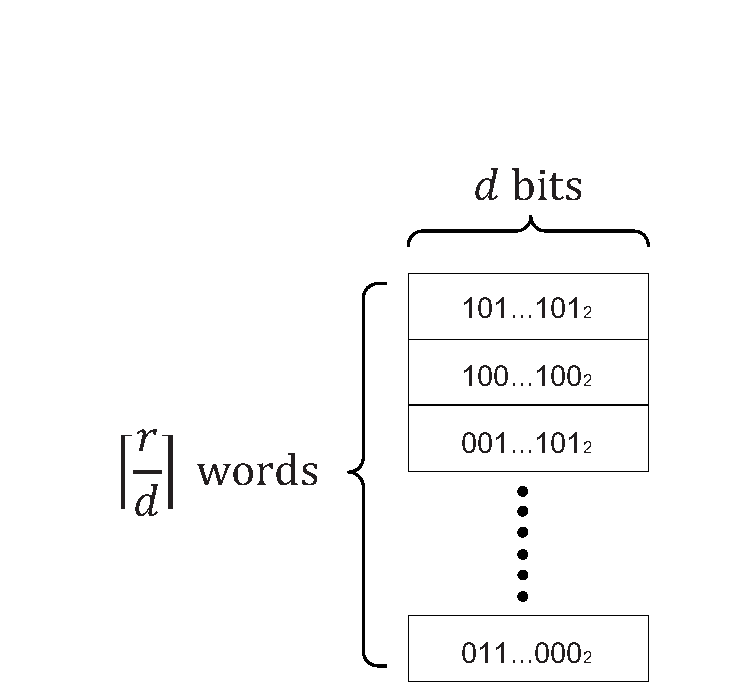
\includegraphics[width=\textwidth]{./fig/PolyDenseFormat.eps}
\caption{Polynomial represented in dense format}
\label{fig:poly_dense}
\end{subfigure}
\hspace{1em}
\begin{subfigure}[t]{0.43\textwidth}\centering
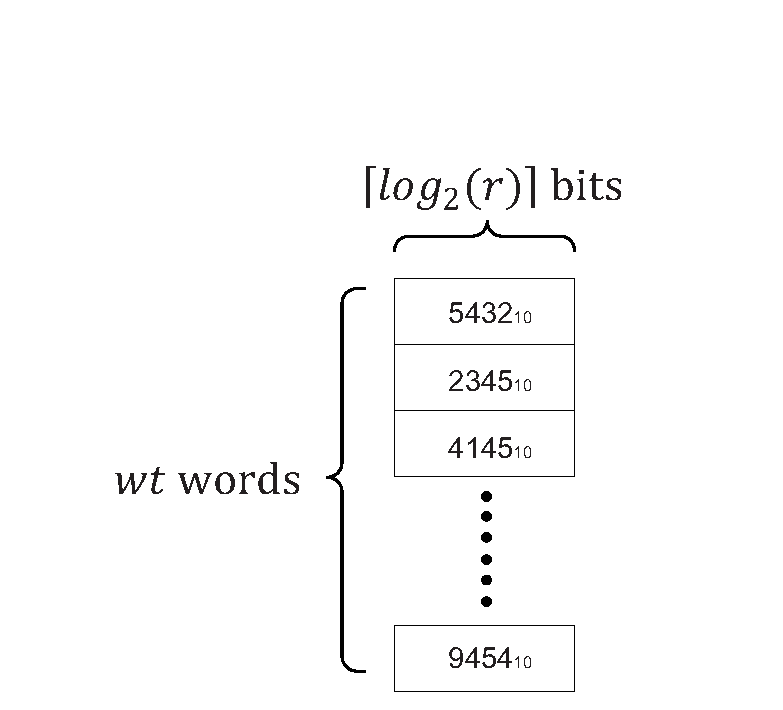
\includegraphics[width=\textwidth]{./fig/PolySparseFormat.eps}
\caption{Polynomial represented in sparse format}
\label{fig:poly_sparse}
\end{subfigure}
\caption{Polynomial in $\mathbb{F}_2[x]/(x^r+1)$ represented in different formats}
\end{figure*}

\subsection{Polynomial Arithmetics}
\subsubsection{Polynomial Inverse}
\begin{figure}[!tb]
\centering
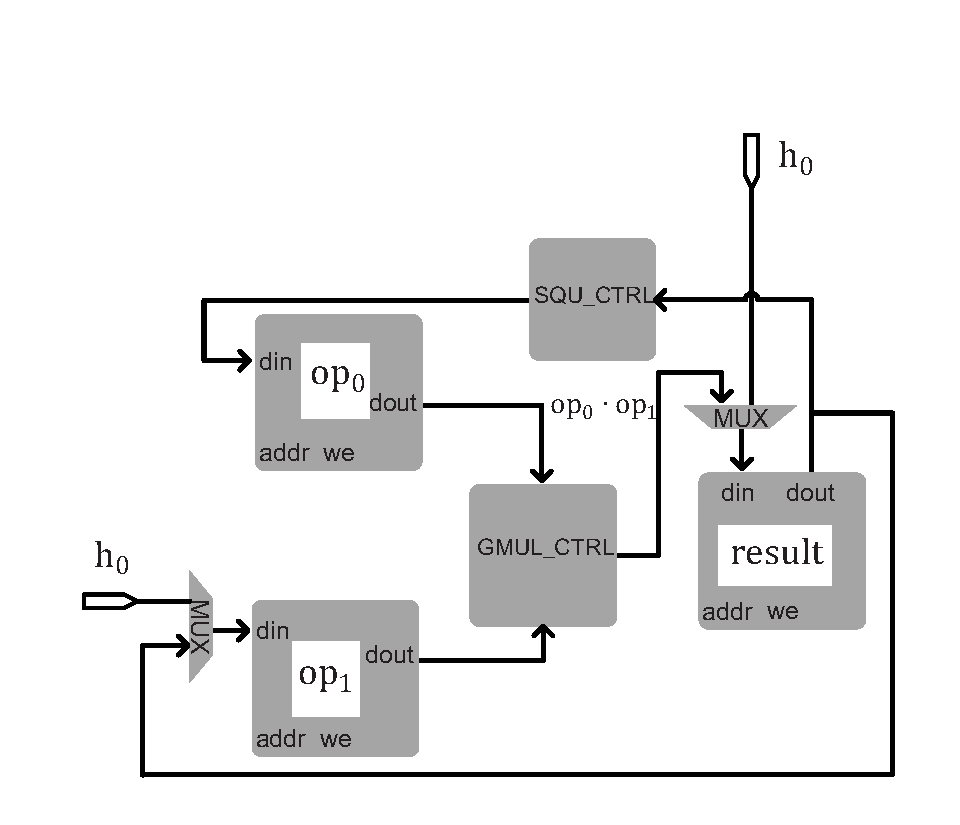
\includegraphics[width=.55\textwidth]{./fig/inv_unit.eps}
\caption{Detailed polynomial inversion architecture}\label{fig:inverter}
\end{figure}

\begin{theorem}
Let $a$ be an invertible polynomial in the quotient ring $\mathbb{F}_2[x]/(x^r+1)$ where $r$ is a prime, then the inverse of polynomial $a$ can be computed as $a^{-1}=(a^{2^{r-2}-1})^2$
\end{theorem}

According to Theorem~1, we can compute the polynomial inverse over ring by exponentiation. Next, we describe our method to fast compute such exponentiation. Let us define the function $\beta_{k}(a)=a^{2^k-1}$, it is easy to see that $a^{-1}=(\beta_{r-2}(a))^2$ in the quotient ring $\mathbb{F}_2[x]/(x^r+1)$. The following recursive
formula holds:
\[
    \beta_{k+j}(a)=(\beta_{k}(a))^{2^j}\beta_{j}(a)
\]

With the recursion above, we can generate $\beta_{r-2}(a)$ from $\beta_{1}(a)=a$ via an addition chain in constant steps, which is known as Itoh-Tsujii Inversion algorithm (ITA). In this paper, we implement the algorithmic description from \cite{hu2015fast} as shown in Alg.~\ref{algo:ITA}. An illustrative example for computing the inverse used in BIKE-2, 128-bit security is listed in Table~\ref{table:ita_example}. From this table, it is seen that ITA is not only fast (20 multiplications + 20 squarings) but also performs in constant time. Fig.~\ref{fig:inverter} depicts the overview of the ITA inverter. The initial polynomial $\beta$ is uploaded to RAM result and raised to ${\beta}^{2^t}$ via SQU\_CTRL which is the module for squaring. This result is then stored to RAM op0. GMUL\_CTRL performs the generic multiplication (step 4,7, Alg.~\ref{algo:ITA}). After the final squaring (step 10), the inverted polynomial appears in RAM op0. In the next subsections, we detail the squaring and the generic multiplication used in ITA.

\begin{algorithm}[!tb]
\DontPrintSemicolon % Some LaTeX compilers require you to use \dontprintsemicolon instead
\KwIn{$r-2=(r_{q-1} \ldots r_0)_2$ and $\alpha \in \mathbb{F}_2[x]/(x^r+1)$.}
\KwOut{$\beta =  \alpha ^{-1}$}
$\beta \gets \alpha$ \;
$t \gets 1$ \;
\For{$i \gets q-2$ \textbf{to} $0$}{
    $\beta \gets (\beta )^{2^{t}} \cdot \beta$\;
    $t \gets 2t$\;
   \uIf{$r_i = 1$}{
        $\beta \gets (\beta)^{2} \cdot  \alpha $\;
        $t \gets t + 1$\;
	  }
}
 $\beta \gets \beta ^2$ \;
\Return {$\beta$}


\caption{Itoh-Tsujii Inversion Algorithm (ITA) \cite{hu2015fast}}
\label{algo:ITA}
\end{algorithm}

\begin{table}[!tb]\centering
\caption{An illustrative example for computing polynomial inverse $a^{-1}$ in $\mathbb{F}_2[x]/(x^r+1)$ with $r=10163$ used in BIKE-2. This table explicitly demonstrates step by step a constat-time execution for inverse.}\scriptsize
\label{table:ita_example}
\begin{tabular}{ccccc}
  \hline
  % after \\: \hline or \cline{col1-col2} \cline{col3-col4} ...
  $i$ & $u_i$ & rule & $[\beta_{u_{i_1}}(a)]^{2^{u_{i_2}}}\cdot \beta_{u_{i_2}}(a)$ & $\beta_{u_{i_i}}(a)=a^{2^{u_i}-1}$\\
  \hline
  0   & 1       & --- & ---                                                         & $\beta_{u_{i_0}}(a)=a^{2^{1}-1}$\\
  1   & 2       & $2u_{i-1}$ &$[\beta_{u_{i_0}}(a)]^{2^{u_{i_0}}}\cdot \beta_{u_{i_0}}(a)$ & $\beta_{u_{i_1}}(a)=a^{2^{2}-1}$\\
  2   & 4       & $2u_{i-1}$ &$[\beta_{u_{i_1}}(a)]^{2^{u_{i_1}}}\cdot \beta_{u_{i_1}}(a)$ & $\beta_{u_{i_2}}(a)=a^{2^{4}-1}$\\
  3   & 8       & $2u_{i-1}$ &$[\beta_{u_{i_2}}(a)]^{2^{u_{i_2}}}\cdot \beta_{u_{i_2}}(a)$ & $\beta_{u_{i_3}}(a)=a^{2^{8}-1}$\\
  4   & 9  & $u_{i-1}+u_0$   &$[\beta_{u_{i_3}}(a)]^{2^{u_{i_0}}}\cdot \beta_{u_{i_0}}(a)$ & $\beta_{u_{i_4}}(a)=a^{2^{9}-1}$\\
  5   & 18       & $2u_{i-1}$ &$[\beta_{u_{i_4}}(a)]^{2^{u_{i_4}}}\cdot \beta_{u_{i_4}}(a)$ & $\beta_{u_{i_5}}(a)=a^{2^{18}-1}$\\
  6   & 19  & $u_{i-1}+u_0$   &$[\beta_{u_{i_5}}(a)]^{2^{u_{i_0}}}\cdot \beta_{u_{i_0}}(a)$ & $\beta_{u_{i_4}}(a)=a^{2^{19}-1}$\\
  7   & 38  & $2u_{i-1}$ &$[\beta_{u_{i_6}}(a)]^{2^{u_{i_6}}}\cdot \beta_{u_{i_6}}(a)$ & $\beta_{u_{i_7}}(a)=a^{2^{38}-1}$\\
  8   & 39  & $u_{i-1}+u_0$   &$[\beta_{u_{i_7}}(a)]^{2^{u_{i_0}}}\cdot \beta_{u_{i_0}}(a)$ & $\beta_{u_{i_8}}(a)=a^{2^{39}-1}$\\
  9   & 78  & $2u_{i-1}$ &$[\beta_{u_{i_8}}(a)]^{2^{u_{i_8}}}\cdot \beta_{u_{i_8}}(a)$ & $\beta_{u_{i_9}}(a)=a^{2^{78}-1}$\\
  10  & 79  & $u_{i-1}+u_0$   &$[\beta_{u_{i_9}}(a)]^{2^{u_{i_0}}}\cdot \beta_{u_{i_0}}(a)$ & $\beta_{u_{i_{10}}}(a)=a^{2^{79}-1}$\\
  11  & 158  & $2u_{i-1}$ &$[\beta_{u_{i_{10}}}(a)]^{2^{u_{i_{10}}}}\cdot \beta_{u_{i_{10}}}(a)$ & $\beta_{u_{i_{11}}}(a)=a^{2^{158}-1}$\\
  12  & 316  & $2u_{i-1}$ &$[\beta_{u_{i_{11}}}(a)]^{2^{u_{i_{11}}}}\cdot \beta_{u_{i_{11}}}(a)$ & $\beta_{u_{i_{12}}}(a)=a^{2^{316}-1}$\\
  13  & 317  & $u_{i-1}+u_0$   &$[\beta_{u_{i_{12}}}(a)]^{2^{u_{i_0}}}\cdot \beta_{u_{i_0}}(a)$ & $\beta_{u_{i_{13}}}(a)=a^{2^{317}-1}$\\
  14  & 634  & $2u_{i-1}$ &$[\beta_{u_{i_{13}}}(a)]^{2^{u_{i_{13}}}}\cdot \beta_{u_{i_{13}}}(a)$ & $\beta_{u_{i_{14}}}(a)=a^{2^{634}-1}$\\
  15  & 635  & $u_{i-1}+u_0$   &$[\beta_{u_{i_{14}}}(a)]^{2^{u_{i_0}}}\cdot \beta_{u_{i_0}}(a)$ & $\beta_{u_{i_{15}}}(a)=a^{2^{635}-1}$\\
  16  & 1270  & $2u_{i-1}$ &$[\beta_{u_{i_{15}}}(a)]^{2^{u_{i_{15}}}}\cdot \beta_{u_{i_{15}}}(a)$ & $\beta_{u_{i_{16}}}(a)=a^{2^{1270}-1}$\\
  17  & 2540  & $2u_{i-1}$ &$[\beta_{u_{i_{16}}}(a)]^{2^{u_{i_{16}}}}\cdot \beta_{u_{i_{16}}}(a)$ & $\beta_{u_{i_{17}}}(a)=a^{2^{2540}-1}$\\
  18  & 5080  & $2u_{i-1}$ &$[\beta_{u_{i_{17}}}(a)]^{2^{u_{i_{17}}}}\cdot \beta_{u_{i_{17}}}(a)$ & $\beta_{u_{i_{18}}}(a)=a^{2^{5080}-1}$\\
  19  & 10160 & $2u_{i-1}$ &$[\beta_{u_{i_{18}}}(a)]^{2^{u_{i_{18}}}}\cdot \beta_{u_{i_{18}}}(a)$ & $\beta_{u_{i_{19}}}(a)=a^{2^{10160}-1}$\\
  20  & 10161 & $u_{i-1}+u_0$ &$[\beta_{u_{i_{19}}}(a)]^{2^{u_{i_{0}}}}\cdot \beta_{u_{i_{0}}}(a)$ & $\beta_{u_{i_{20}}}(a)=a^{2^{10161}-1}$\\
  \hline
\end{tabular}
\end{table}


\subsubsection{Squaring in $\mathbb{F}_2[x]/(x^r+1)$}
First, consider the direct squaring $a^2(x)$ for any polynomial $a(x)\in \mathcal{R}$:
\begin{align}
    a^2(x) &= (a_{r-1}x^{r-1}+a_{r-2}x^{r-2}+\cdots + a_{1}x + a_0)^2\\
    &= a_{r-1}x^{2(r-1)}+a_{r-2}x^{2(r-2)}+\cdots + a_1x^2 + a_0\\
    &= \widetilde{a_{r-1}}x^{r-1}+\widetilde{a_{r-2}}x^{r-2}+\cdots + \widetilde{a_{1}}x +\widetilde{a_0}
\end{align}

To compute the coefficients $\widetilde{a_{i}}$, the matrix multiplication is used, the key is the base transformation matrix BT, shown as follows:
\[
a^2(x)= [{a_{0}},{a_{1}},\cdots,{a_{r-1}}]\left[ \begin{array}{c}
x^{0} \\
x^{2} \\
\vdots\\
x^{2(r-2)}\\
x^{2(r-1)}
\end{array}
\right ]
=
[{a_0},{a_1},\cdots,{a_{r-1}}]
\cdot \text{BT}_{r\times r} \cdot
\left[ \begin{array}{c}
x^{0} \\
x^{1} \\
\vdots\\
x^{r-2}\\
x^{r-1}
\end{array}
\right ]
\]
where $[\widetilde{a_{0}},\widetilde{a_{1}},\cdots,\widetilde{a_{r-1}}]=[{a_{0}},{a_{1}},\cdots,{a_{r-1}}]
\cdot \text{BT}$ and BT is a $r\times r$ permutation matrix defined as:
\[
\text{BT} =
\left[ \begin{array}{ccccc}
\mathbf{1}_{0}&0&\cdots&\cdots&\cdots  \\
\cdots&\mathbf{1}_{2}&0 &\cdots&\cdots \\
\vdots&\vdots&\vdots&\vdots&\vdots\\
\vdots&\vdots&\mathbf{1}_{2r-4}&0&\vdots\\
\vdots&\vdots&\vdots&\mathbf{1}_{2r-2}&0\\
\end{array}
\right ]
\]
where $\mathbf{1}_{i}$ represents the ($i\bmod r$)-th (counting from zero) non-zero entry in the corresponding row of the matrix BT.

More generally, we derive the base transformation matrix $\text{BT}_n=\text{BT}^n$ for continuous square $a(x)^{2^n}=\widetilde{a_{r-1}}x^{r-1}+\widetilde{a_{r-2}}x^{r-2}+\cdots + \widetilde{a_{1}}x +\widetilde{a_0}$, which is particularly useful in computing the polynomial inverse.
\[
\text{BT}^n =
\left[ \begin{array}{ccccc}
\mathbf{1}_{0}&0&\cdots&\cdots&\cdots  \\
\cdots&\mathbf{1}_{2^n}&0 &\cdots&\cdots \\
\vdots&\vdots&\vdots&\vdots&\vdots\\
\vdots&\vdots&\mathbf{1}_{(r-2)2^n}&0&\vdots\\
\vdots&\vdots&\vdots&\mathbf{1}_{(r-1)2^n}&0\\
\end{array}
\right ]
\]

In order to compute the coefficient vector $[\widetilde{a_{0}},\widetilde{a_{1}},\cdots,\widetilde{a_{r-1}}]=[{a_{0}},{a_{1}},\cdots,{a_{r-1}}]
\cdot \text{BT}^n$, $\text{BT}^n$ must be represented in column view, \textit{i.e.},
the row number of the non-zero entry for every column of $\text{BT}^n$.
\[
\text{BT}^n =
\left[ \begin{array}{ccccc}
\mathbf{1}_{0}&\vdots& \vdots&\vdots&\vdots \\
\vdots&\mathbf{1}_{2^{-n}}&\vdots&\vdots&\vdots\\
\vdots&\vdots&\vdots&\mathbf{1}_{(r-2)2^{-n}}&\vdots\\
\vdots&\vdots&\vdots&\vdots&\mathbf{1}_{(r-1)2^{-n}}\\
\end{array}
\right ]
\]

In other terms, each $\widetilde{a_{i}}$ is updated by $a_{j}$ in $[{a_{r-1}},{a_{r-2}},\cdots,{a_0}]$ as:
\[
    \widetilde{a_{i}} = a_{i2^{-n}\bmod r}
\]

Note that the data is typically processed digit by digit on hardware. However, sometimes we want to extract the precise bit in the digit. Squaring is such an example where the result is indeed computed bit by bit. To preserve the constant time execution while avoiding the timing performance degration, Barrel shifter is used to rotate the desired bit within $\lceil log_2d\rceil$ cycles.

Fig.~\ref{fig:pipeline_squ} depicts the pipeline stages for computing the continuous square. The basic pattern is: read from memory the entry which contains $a_{i2^{-n}}$, then load it to the Barrel shifter, rotate to correct bit position, and finally write the result back to memory. In general, such pattern repeats $r$ times and hence the cycle counts for continuous square are
\[
    r(\lceil log_2d\rceil+3)
\]
Next, the above pipeline can be further improved based on the observation that read and rotate can be parallelized, and load and write can be parallelized as well. To sum up, the optimized cycle counts are
\[
    r(\lceil log_2d\rceil+1)+2
\]


\begin{figure*}[!tb]
\centering
\begin{subfigure}[t]{0.5\textwidth}\centering
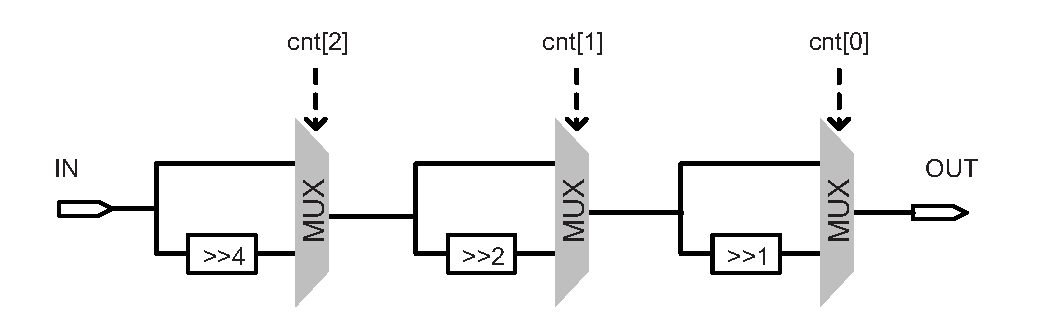
\includegraphics[width=\textwidth]{./fig/barrel1.eps}
\caption{Barrel shifter constructed by combinational logic}
\label{fig:L1_ctrl}
\end{subfigure}
\hspace{1em}
\begin{subfigure}[t]{0.4\textwidth}\centering
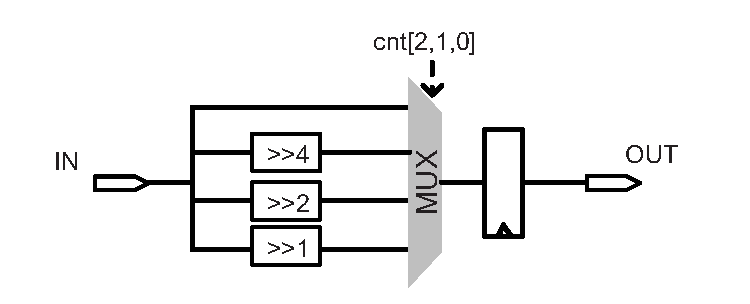
\includegraphics[width=\textwidth]{./fig/barrel2.eps}
\caption{Barrel shifter constructed by sequential logic}
\label{fig:FLIP_ctrl}
\end{subfigure}
\caption{Barrel shifter used in our key generator to ensure constant execution of multiplication and squaring}
\end{figure*}

\begin{figure*}[!tb]
\centering
\begin{subfigure}[t]{0.45\textwidth}\centering
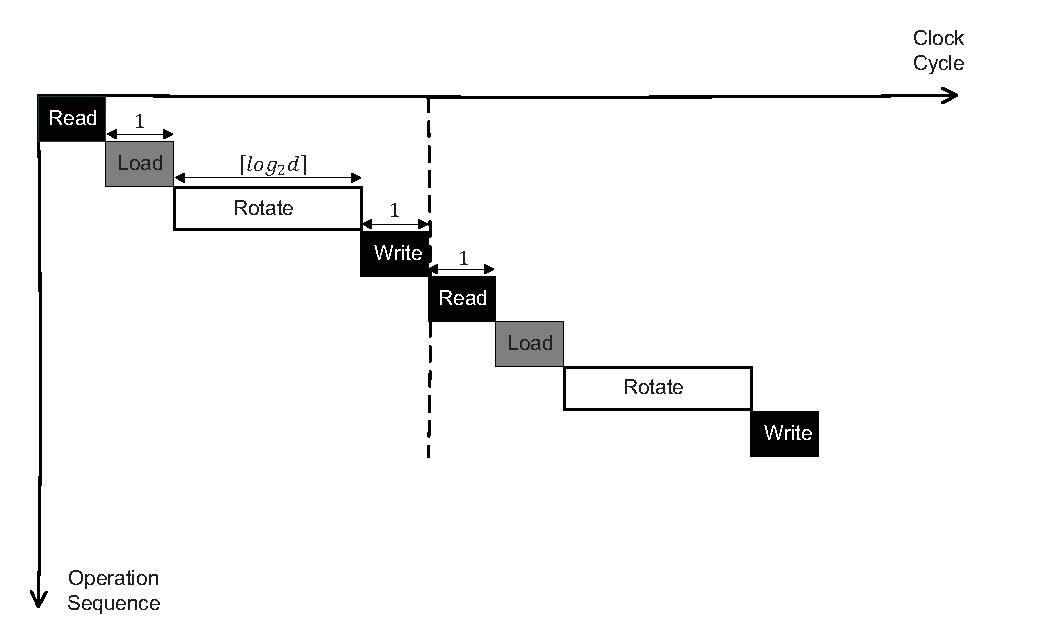
\includegraphics[width=\textwidth]{./fig/pipeline_square.eps}
\caption{Primitive operation pipelining for continuous square}
\label{fig:pipeline_squ}
\end{subfigure}
\hspace{1em}
\begin{subfigure}[t]{0.45\textwidth}\centering
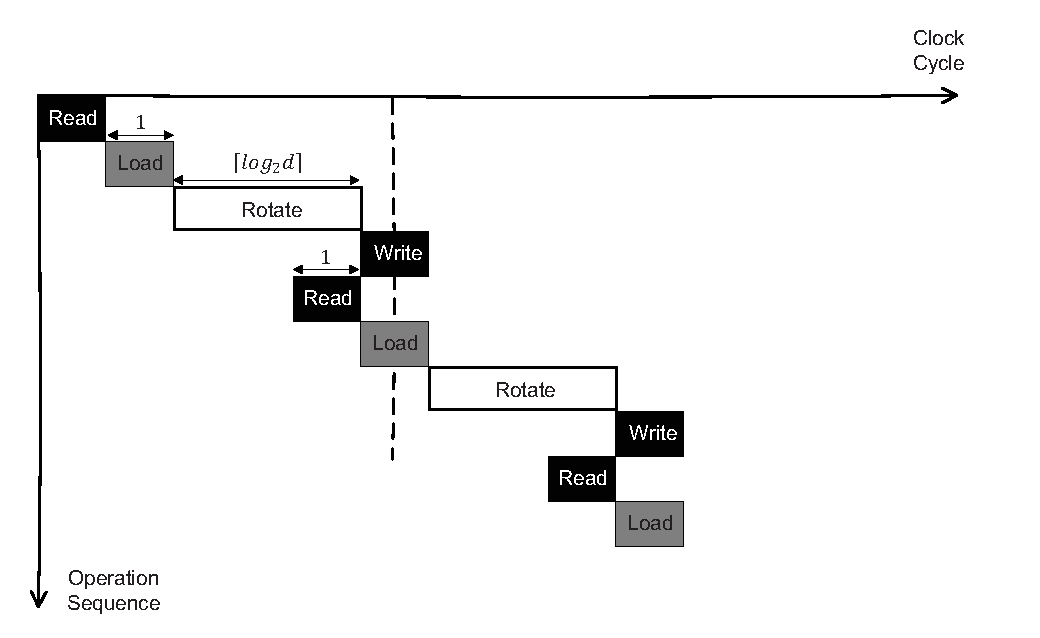
\includegraphics[width=\textwidth]{./fig/pipeline_square2.eps}
\caption{Optimised operation pipelining for continuous square }
\label{fig:pipeline_squ2}
\end{subfigure}
\caption{Timing diagram used in continuous square}
\end{figure*}


\subsubsection{Generic Multiplication in $\mathbb{F}_2[x]/(x^r+1)$}
For two dense polynomials $a(x)$ and $b(x)$, their multiplication is represented as:
\begin{align}
    a(x)\cdot b(x) &= (a_{r-1}x^{r-1}+\cdots + a_{1}x + a_0)\cdot(b_{r-1}x^{r-1}+\cdots + b_{1}x + b_0)\\
    &= \widetilde{c_{r-1}}x^{r-1}+\widetilde{c_{r-2}}x^{r-2}+\cdots + \widetilde{c_{1}}x +\widetilde{c_0}
\end{align}

Likewise, another base transformation matrix $\text{BT}_{mul}$ is used to compute the coefficients $\widetilde{c_{i}}$ of $a(x)b(x)$, shown as follows:
\[
a(x)b(x)= [\widetilde{c_{0}},\widetilde{c_{1}},\cdots,\widetilde{c_{r-1}}]\left[ \begin{array}{c}
x^{0} \\
x^{1} \\
\vdots\\
x^{r-2}\\
x^{r-1}
\end{array}
\right ]
=
[{a_{0}},{a_{1}},\cdots,{a_{r-1}}]
\cdot \text{BT}_{mul,r\times r} \cdot
\left[ \begin{array}{c}
x^{0} \\
x^{1} \\
\vdots\\
x^{r-2}\\
x^{r-1}
\end{array}
\right ]
\]
$\text{BT}_{mul}$ is a $r\times r$ matrix where each column/row is a cyclic form of the vector $[b_{r-1},b_{r-2},\ldots, b_{1},b_{0}]$:
\[
\text{BT} =
\left[ \begin{array}{cccccc}
b_{0}&b_{1}&\cdots&b_{d-1}&\cdots &b_{r-1} \\
b_{r-1}&b_{0}&\cdots&b_{d-2}&\cdots &b_{r-2} \\
\vdots&\vdots&\vdots&\vdots&\vdots&\vdots\\
b_{2}&b_{3}&\cdots&b_{d+1}&\cdots &b_{1} \\
b_{1}&b_{2}&\cdots&b_{d}&\cdots &b_{0} \\
\end{array}
\right ]
\]
BT is redundant since the blocks along each diagonal is identical (for example, $BT[0:d-1,0:d-1] = BT[d:2d-1,d:2d-1] = \ldots$). This way, BT is split into three parts: the central diagonal, the upper triangle, and the lower triangle. Fig.~\ref{fig:gmul_ill1}, \ref{fig:gmul_ill2}, and \ref{fig:gmul_ill3} illustrate how to compute them. By eliminating such redundancy, the communication overhead for loading $\text{BT}_{mul}$ is minimized and therefore, faster pipeline scheduling is possible in the generic multiplication.

A formal description for the proposed generic multiplication can be found in Alg.~\ref{alg:generic_mul}. It is seen that the core function is the multiplication of a $d$-bit vector $A[k]$ of $a(x)$ and a block matrix BT$[i,j]$ from BT:
\[
    [a_j,a_{j+1},\ldots,a_{j+d-1}]\cdot
\left[ \begin{array}{ccccc}
b_{i}&b_{i+1}&b_{i+2}&\cdots &b_{i+d-1} \\
b_{i-1}&b_{i}&b_{i+1}&\cdots &b_{i+d-2} \\
\vdots&\vdots&\vdots&\vdots&\vdots\\
b_{i-d+1}&b_{i-d+2}&b_{i-d+3}&\cdots &b_{i} \\
\end{array}
\right ]_{d\times d}
\]
We design a dedicate core unit for the multiplication above in one clock cycle, depicted in Fig~\ref{fig:gmul_core}. With this module, the proposed generic multiplication algorithm can be scheduled as Fig.~\ref{fig:pipeline_gmul} shows. Read takes 5 cycles to balance the critical path for reading $B[i,j]$. Again the dual-port RAM is used such that the target vector $B[i,j]$ can be loaded within two cycles. Here a fixed rotation is performed to move $A[k]$ to the correct bit positions. MUL performs the core multiplication $A[k]\cdot B[i,j]$ and later writes back the result.

\begin{algorithm}[!tbh]
 \DontPrintSemicolon % Some LaTeX compilers require you to use \dontprintsemicolon instead
 \KwIn{dense polynomials $a(x),b(x) \in \mathbb{F}_2[x]/(x^r+1)$.}
 \KwOut{$a(x)\cdot b(x)\in \mathbb{F}_2[x]/(x^r+1)$}
    Reformulate $a(x)$ to block matrix view as $A[0],A[1],A[2],\ldots, A[n-1]$ where $n=\lceil r/d \rceil$, $d$ is the number of bits used in the row vector $A[i]$.\;
    Compute partial blocks from the transformation matrix BT associated with $b(x)$: $BT[0,0]$, $BT[0,1],BT[0,2],\ldots,BT[0,n-1]$ and $BT[1,0]$, $BT[2,0],\ldots,BT[n-1,0]$\;
    The multiplication result is presented again in block matrix view $C[0],C[1],C[2],\ldots, C[n-1]$\;
    /*Diagonal Computation*/\;
    \For{$i \gets 0 \textbf{ to } n-1$}{
        $C[i] \gets A[i]\cdot BT[0,0]$\;
    }
    /*Upper Triangle Computation*/\;
    \For{$i \gets 1 \textbf{ to } n-1$}{
        \For{$j \gets 0 \textbf{ to } n-1-i$}{
           $C[i+j] \gets C[i+j] + A[j]\cdot BT[0,i]$\;
        }
    }
    /*Lower Triangle Computation*/\;
    \For{$i \gets 1 \textbf{ to } n-1$}{
        \For{$j \gets 0 \textbf{ to } n-1-i$}{
           $C[j] \gets C[j] + A[i+j]\cdot BT[i,0]$\;
        }
    }
    \Return {the vector $C=[C[0],C[1],\ldots,C[n-1]]$ as the coefficients of $c(x)=a(x)b(x)$\;}
 \caption{Proposed generic multiplication algorithm}\label{alg:generic_mul}
\end{algorithm}


%\begin{table}[!tb]\centering
%\caption{Cycle counts for computing one block in Generic Multiplication}
%\begin{tabular}{c|c|c|c}
%  \hline
%  % after \\: \hline or \cline{col1-col2} \cline{col3-col4} ...
%  Operation & Load & Rotate & Mul  \\\hline
%   & 5 & 2 & 1  \\
%  \hline
%\end{tabular}
%\end{table}


\begin{figure*}[!tb]
\centering
\begin{subfigure}[t]{0.47\textwidth}\centering
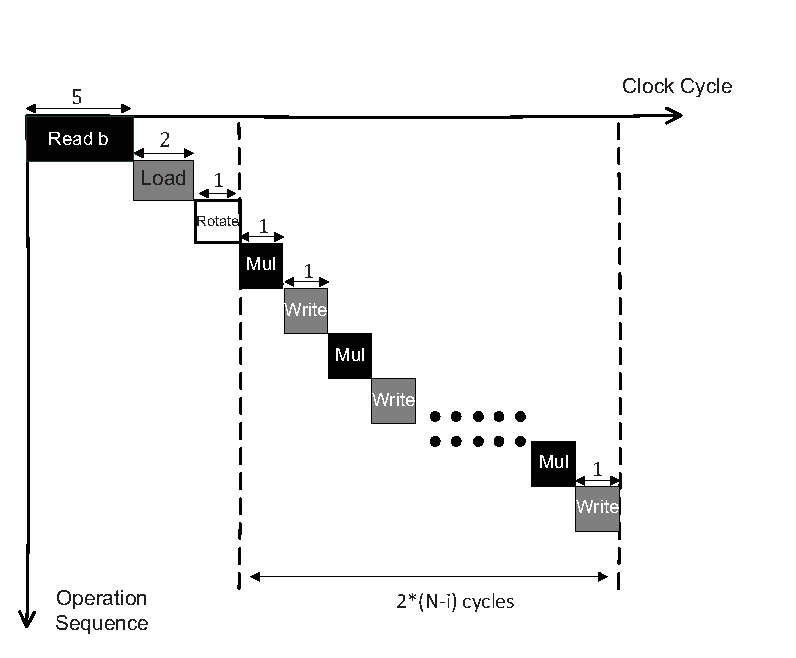
\includegraphics[width=\textwidth]{./fig/pipeline_dsnmul.eps}
\caption{Primitive operation pipelining for generic multiplication}
\label{fig:pipeline_gmul}
\end{subfigure}
\hspace{1em}
\begin{subfigure}[t]{0.47\textwidth}\centering
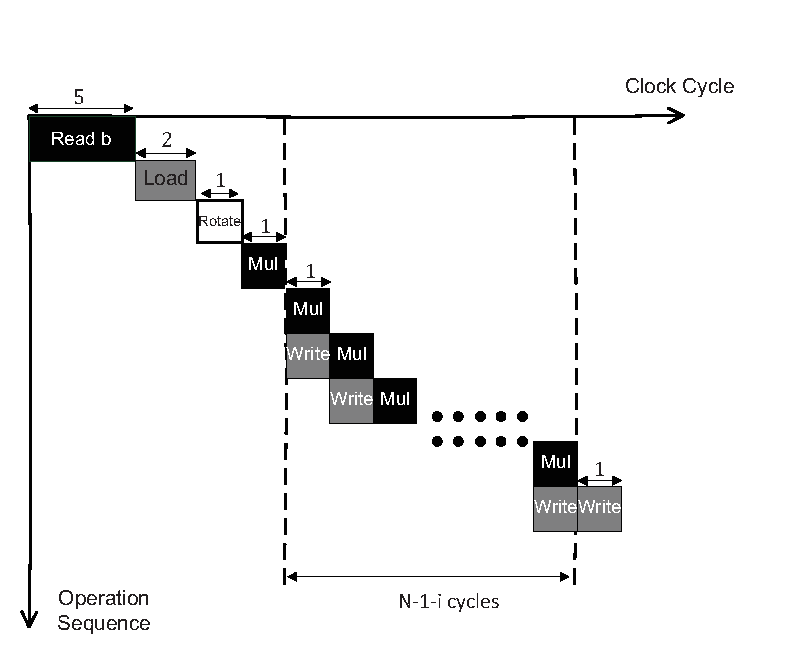
\includegraphics[width=\textwidth]{./fig/pipeline_dsnmul2.eps}
\caption{Optimised operation pipelining for generic multiplication }
\label{fig:pipeline_gmul2}
\end{subfigure}
\caption{Timing diagram used in generic multiplication}
\end{figure*}


\begin{figure*}[!tb]
\centering
\begin{subfigure}[t]{0.45\textwidth}\centering
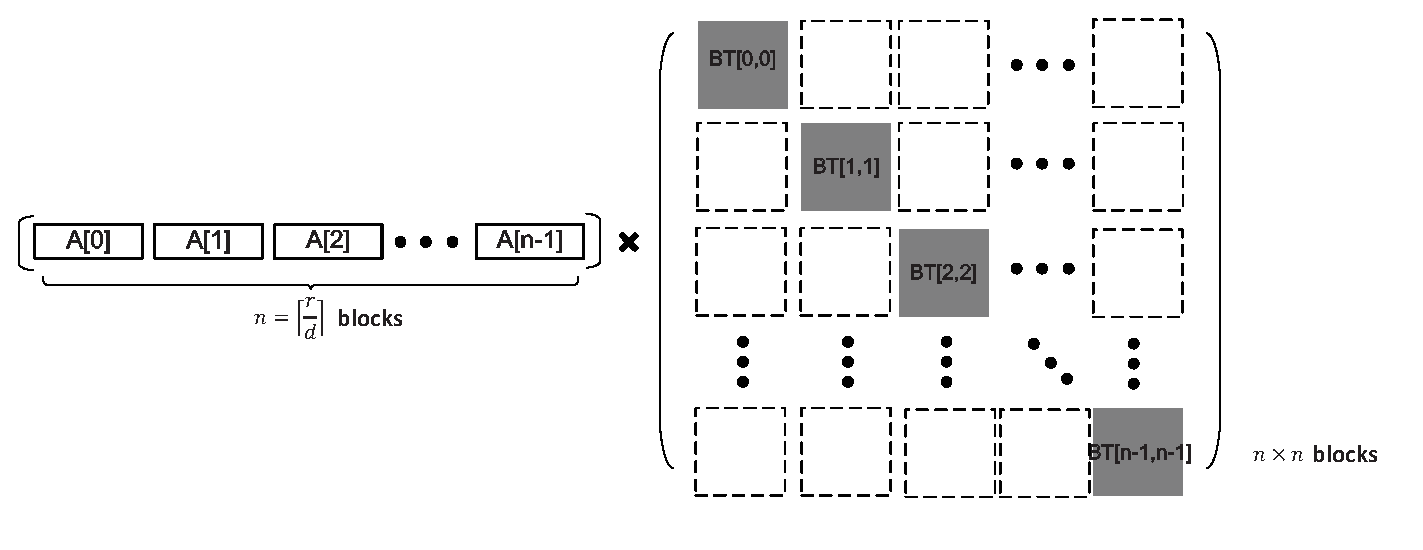
\includegraphics[width=\textwidth]{./fig/generic_mul_illustrate.eps}
\caption{Diagonal Computation}
\label{fig:gmul_ill1}
\end{subfigure}
\hspace{1em}
\begin{subfigure}[t]{0.45\textwidth}\centering
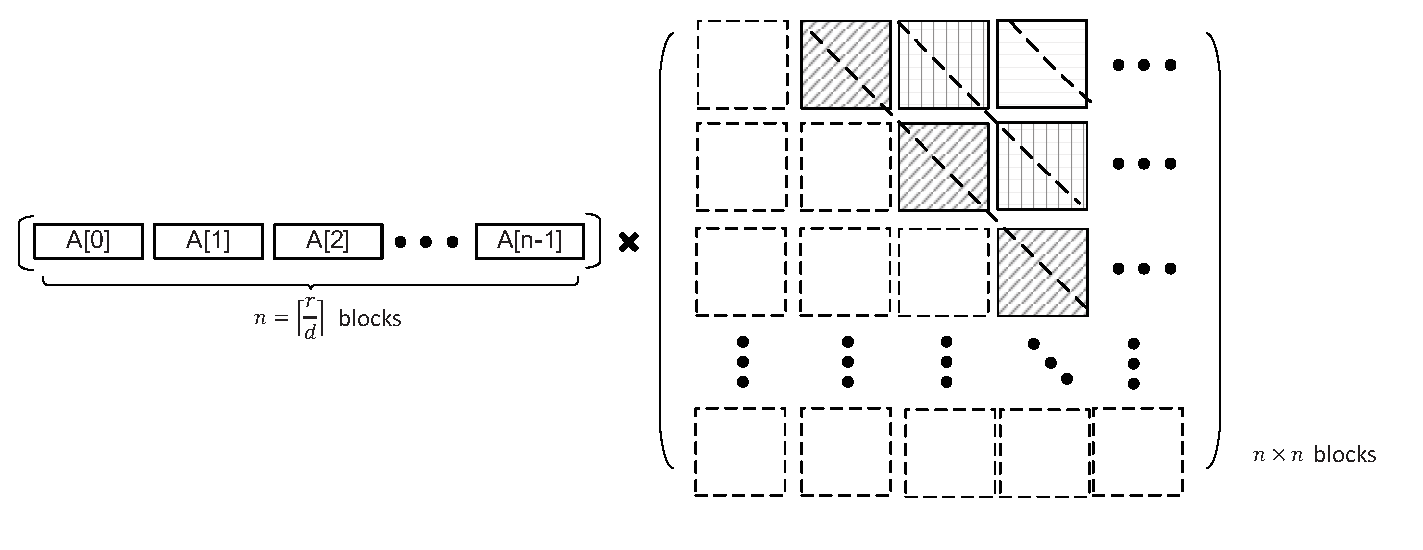
\includegraphics[width=\textwidth]{./fig/generic_mul_illustrate2.eps}
\caption{Upper Triangle Computation}
\label{fig:gmul_ill2}
\end{subfigure}
\hspace{1em}
\begin{subfigure}[t]{0.45\textwidth}\centering
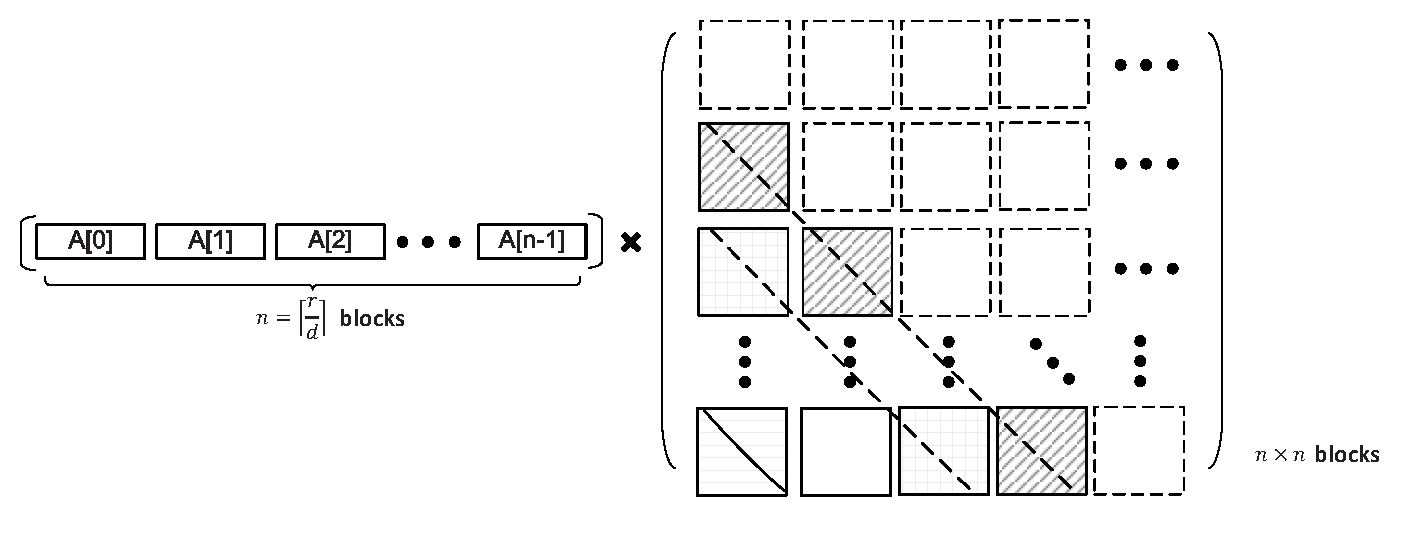
\includegraphics[width=\textwidth]{./fig/generic_mul_illustrate3.eps}
\caption{Lower Triangle Computation}
\label{fig:gmul_ill3}
\end{subfigure}
\caption{Illustration for the proposed generic multiplication algorithm}
\end{figure*}


\begin{figure}[!tb]
\centering
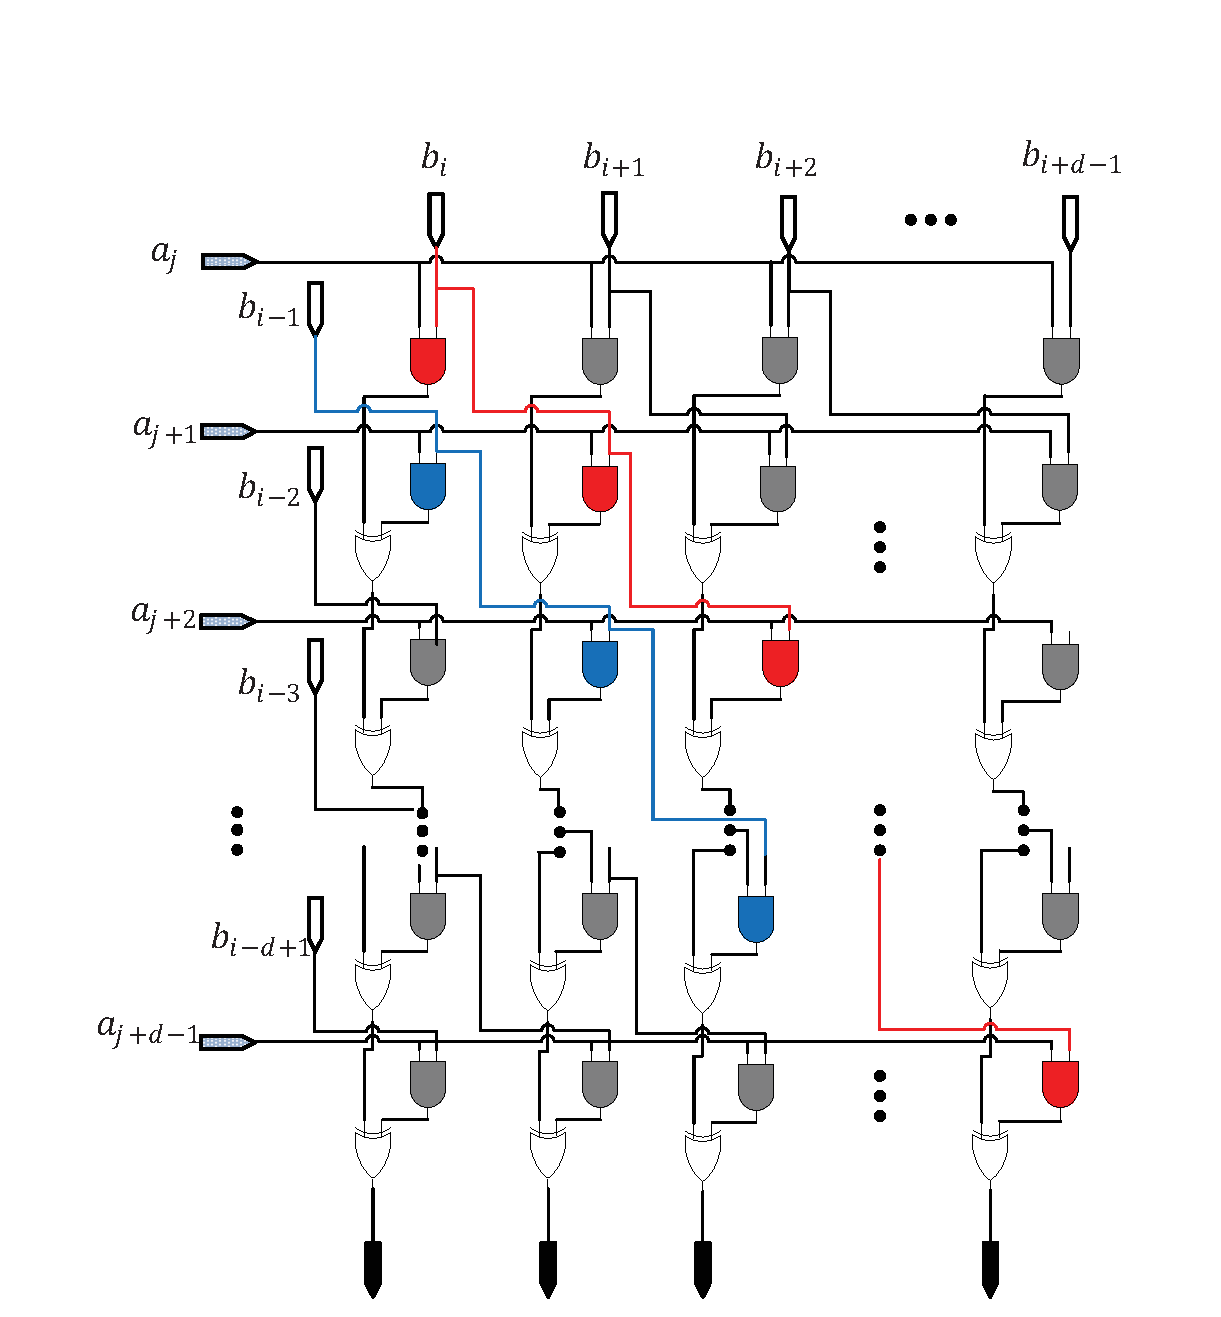
\includegraphics[width=.55\textwidth]{./fig/dsnmul_core.eps}
\caption{architectural overview of the core unit in the generic multiplication}\label{fig:gmul_core}
\end{figure}

An even better schedule is depicted in Fig.~\ref{fig:pipeline_gmul2} where Mul and Write perform simultaneously.
To handle the diagonal computation, it takes $5+2+1+2\lceil r/d\rceil$ cycle counts where $i=0$. $\lceil r/d\rceil -1$ iterations are required for the upper triangle computation. A particular $i=1,2,\ldots,d-1$-th iteration consumes $5+2+1+\lceil r/d\rceil -1-i+1$ cycle counts and thus the entire upper triangle computation costs $(\lceil r/d\rceil^2 +17\lceil r/d\rceil-18)/2$ cycle counts. The same cycle counts are needed for the lower triangle computation.

In general, the optimised cycle counts for generic multiplication are
\[
    \lceil r/d\rceil^2 + 18\lceil r/d\rceil - 9
\]

\subsection{Sparse-Times-Dense Multiplication in $\mathbb{F}_2[x]/(x^r+1)$}
In BIKE, a special form of multiplication called sparse-times-dense multiplication, is frequently used. In sparse-times-dense multiplication, one of the operands is a sparse polynomial whereas the other is a dense polynomial. Such multiplication can be efficiently computed as follows: The sparse polynomial, \textit{e.g}, $a(x)$ is first represented by an array of indices in $I=\{i|a_i=1\}$. Then, the multiplication result can be obtained by extracting $i\in I$ rows of $\text{BT}_{mul}$ and then accumulating them, \textit{i.e.}, $\sum_{i\in I} x^ib(x)$ and the $i$-th row of the matrix $\text{BT}_{mul}$ represents the coefficients of $x^ib(x)$. Formally, the coefficient vector of sparse-times-dense multiplication can be calculated as follows:
\[
    \sum_{i\in I} [b_{-i},b_{-i+1},\cdots,b_{-i-1}]
\]

\begin{table}[!tb]\centering
\caption{Cycle counts for extracting $d$ bits of $x^ib(x)$ in Sparse-Times-Dense Multiplication}
\begin{tabular}{c|c|c|c|c|c|c|c}
  \hline
  % after \\: \hline or \cline{col1-col2} \cline{col3-col4} ...
  Operation & Read\_h & Read\_g & Load &Rotation & Add & Write & Total \\\hline
   & 3 & 3 & 2 & $\lceil log_2(d)\rceil$ & 1 & 1& 10+$\lceil log_2(d)\rceil$ \\
  \hline
\end{tabular}
\end{table}

Fig.~\ref{fig:pipeline_mul} depicts the basic pipeline schedule where the total cycle counts for one complete sparse-times-dense multiplication are
\[
    |I|\cdot\lceil r/d\rceil\cdot (10+\lceil log_2(d)\rceil)
\]
and optimized cycle counts are
\[
    |I|(\lceil r/d\rceil\cdot (2+\lceil log_2(d)\rceil) + 8)
\]

\begin{table}[!tb]\centering
\caption{Cycle counts comparison between unoptimized and optimized sparse-times-dense multiplication. The pipelined architecture introduces about 50\% reduction of cycle counts for all BIKE instances}
\begin{tabular}{cc|ccccc}
  \hline
  % after \\: \hline or \cline{col1-col2} \cline{col3-col4} ...
 \textbf{Category}        &             & $d$ & $r$  & $|I|=w/2$  & unoptimized version& optimized version\\\hline
\multirow{ 2}{*}{128-bit} &  BIKE-[1,2] & $64$ & $10163$  & $71$  & $180,624$ & $90,880$\\
                          &  BIKE-[3] & $64$ & $11027$  & $67$  & $185,456$& $93,264$\\
  \hline
\multirow{ 2}{*}{192-bit} &  BIKE-[1,2] & $64$ & $19853$  & $103$  &$512,528$& $257,088$\\
                          &  BIKE-[3] & $64$ & $21683$  & $99$  &$536,976$& $269,280$\\
  \hline
\multirow{ 2}{*}{256-bit} &  BIKE-[1,2] & $64$ & $32749$  & $137$  &$1,122,304$& $562,248$\\
                          &  BIKE-[3] & $64$ & $36131$  & $133$  &$2,404,640$& $1,203,384$\\
  \hline
\end{tabular}
\end{table}


\begin{figure*}[!tb]
\centering
\begin{subfigure}[t]{0.5\textwidth}\centering
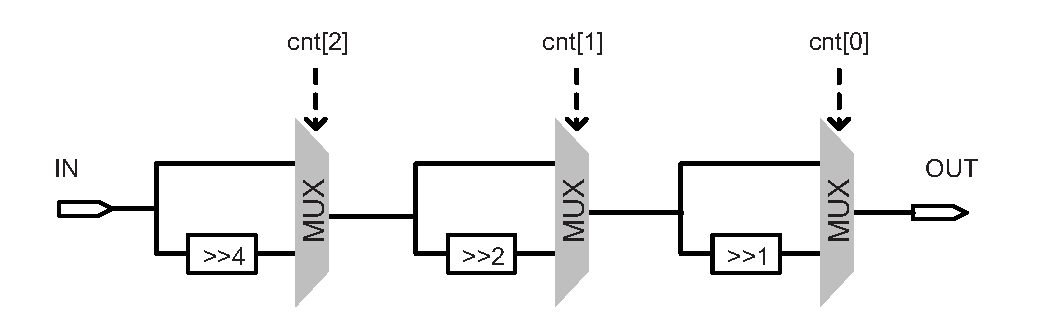
\includegraphics[width=\textwidth]{./fig/barrel1.eps}
\caption{Barrel shifter constructed by combinational logic}
\label{fig:L1_ctrl}
\end{subfigure}
\hspace{1em}
\begin{subfigure}[t]{0.4\textwidth}\centering
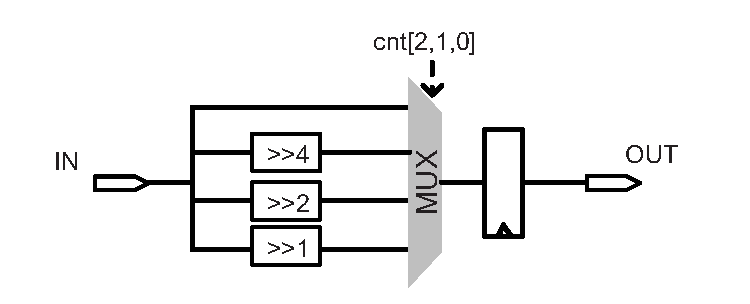
\includegraphics[width=\textwidth]{./fig/barrel2.eps}
\caption{Barrel shifter constructed by sequential logic}
\label{fig:FLIP_ctrl}
\end{subfigure}
\caption{Barrel shifter used in our key generator to ensure constant execution of multiplication and squaring}
\end{figure*}

\begin{figure*}[!tb]
\centering
\begin{subfigure}[t]{0.45\textwidth}\centering
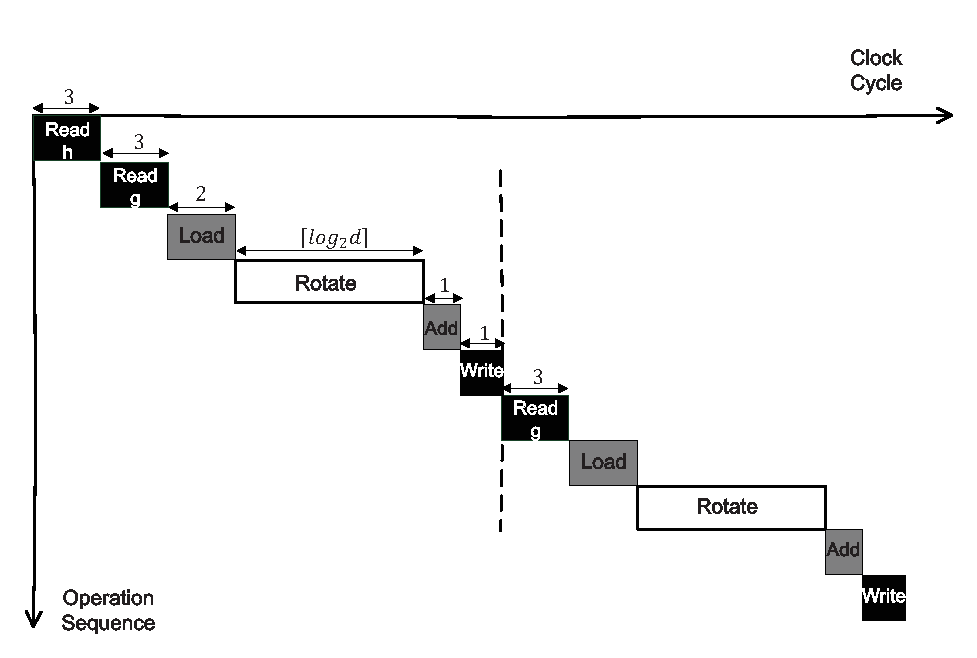
\includegraphics[width=\textwidth]{./fig/pipeline_mul.eps}
\caption{Primitive operation pipelining for sparse-times-dense multiplication}
\label{fig:pipeline_mul}
\end{subfigure}
\hspace{1em}
\begin{subfigure}[t]{0.45\textwidth}\centering
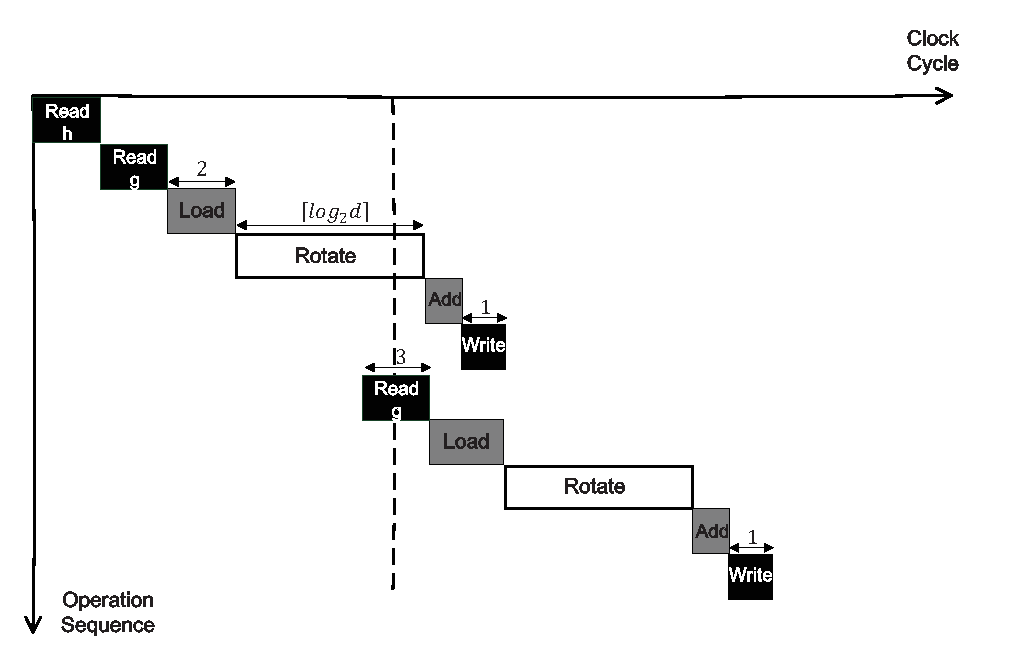
\includegraphics[width=\textwidth]{./fig/pipeline_mul2.eps}
\caption{Optimised operation pipelining for sparse-times-dense multiplication }
\label{fig:pipeline_mul2}
\end{subfigure}
\caption{Timing diagram used in sparse-times-dense multiplication}
\end{figure*}

\subsection{Generation of Polynomials in $\mathbb{F}_2[x]/(x^r+1)$ with Prescribed Weight}

\begin{algorithm}[!tb]
\DontPrintSemicolon % Some LaTeX compilers require you to use \dontprintsemicolon instead
\KwIn{PRNG seed, polynomial length $r$, data width $d$}
\KwOut{binary vector $\mathbf{ \overline{f}}$ representing $f=f_0+\ldots +f_{r-1}x^{r-1}\in \mathbb{F}_2[x]/(x^r+1)$, with odd weight $|f|\approx r/2$}
$wt \gets 0$\;
\For{$i \gets 0 \textbf{ to } \lceil r/d\rceil-1$}{
    $\overline{\mathbf{f}[i]} \gets \text{truncate}_{d}(SecureRand(seed))$\;
    $wt \gets wt+|\overline{\mathbf{f}[i]}|$
}
\uIf{$wt$ is even}{
        flip the first bit in $\overline{\mathbf{f}[i]}$
	  }
\Return {$\overline{\mathbf{f}}$}


\caption{Generation of a random polynomial with odd weight}
\label{alg:prng1}
\end{algorithm}

\SetKwRepeat{Do}{do}{while}%
\begin{algorithm}[!tb]
\DontPrintSemicolon % Some LaTeX compilers require you to use \dontprintsemicolon instead
\KwIn{PRNG seed, polynomial length $r$, data width $d$, polynomial weight $wt=w/2$}
\KwOut{ integer vector $\mathbf{ \hat{f}}$ contains non-zero bit-positions ($\{i|f_i\neq 0\}$  to represent $f=f_0+\ldots +f_{r-1}x^{r-1}\in \mathbb{F}_2[x]/(x^r+1)$, with odd weight $|f|= wt$}
\For{$i \gets 0 \textbf{ to } wt-1$}{
    \Do{$rand \geq r$ or  $rand \in \mathbf{\hat{f}}$ }{
      $rand \gets \text{truncate}_{d}(SecureRand(seed))$\;
    }
    $\mathbf{ \hat{f}}[i] \gets rand$
}
\Return {$\mathbf{ \hat{f}}$}


\caption{Generation of a random sparse polynomial with given (odd) weight}
\label{alg:prng2}
\end{algorithm}

Strictly speaking, the execution of the random polynomial generations proposed in Alg.~\ref{alg:prng1},\ref{alg:prng2} is non-constant. Alg.~\ref{alg:prng1} performs an optional step if the Hamming weight of the polynomial is an even number; Alg.~\ref{alg:prng2} keeps generating new random numbers unless the number is smaller than the system parameter $r$ and non-repeating. Nevertheless, we validate that these non-constant behaviors do not leak any useful information on secrets for an adversary to exploit: The optional step in Alg.~\ref{alg:prng1} flips the first bit-position of $\mathbf{\overline{f}}$ and the probabilistic distribution of this bit position does not change as long as the PRNG itself is unbiased (uniformly distributed). An adversary has no advantage to estimate the value of this specific bit even if he knows the timing difference. For Alg.~\ref{alg:prng2}, the timing difference observed by an adversary is actually the total amount of time introduced by re-generation of random numbers if overflow ($rand\geq r$) or repetition ($rand\in \mathbf{\hat{f}}$) occurs. Overflow does not leak any information about $\mathbf{\hat{f}}$ as overflow only suggests the generated number is above $r$ which leaks no information on $\mathbf{\hat{f}}$. The probability that the generated random number is smaller than $r$ is $Pr(\text{rand} < r)= r/2^{\lceil log_2(r)\rceil}$. To eliminate the possible timing leakage from the repetition, we introduce a method in which we change the while-loop in step 4 to while $rand\geq r$. In other terms, we generate $w_t$ random numbers of which each is smaller than $r$ without considering whether they collide or not. By doing this, no timing information is leaked on repetition but we might occur a few repetitions which reduce the Hamming weight of the sparse polynomial generated. However, a few repetitions are tolerable because BIKE is not sensitive to a slight loss of Hamming weight $w$. To reach $\lambda$ bits of classical security, $\lambda\approx w-log_2r$ for BIKE-1 and BIKE-2 and $\lambda\approx w-\frac{1}{2}log_2r$ for BIKE-3, and 1 or 2 repetitions only decrease the security level $2^\lambda$ to $2^{\lambda-2}$.
More importantly, the probability that a single run of Alg.~\ref{alg:prng2} without considering collision succeeds if we tolerate one or two repetitions is very high (at least 0.997, data are collected in Table~\ref{table:success_rate}):
\begin{align}
    Pr(\text{Alg.~\ref{alg:prng2} succeeds}) &= Pr(\text{0 or 1 or 2 repetition occur})\\
    &=\frac{r(r-1)\cdots (r-w_t+1)}{r^{w_t}}+ \frac{\binom{w_t}{2}r(r-1)\cdots (r-w_t+2)}{r^{w_t}}\\
    &+ \frac{[\binom{w_t}{3}+\binom{w_t}{2}\binom{w_t-2}{2}/2]  r(r-1)\cdots (r-w_t+3) }{r^{w_t}}
\end{align}

%Now assume $t$ (typically small compared with $wt$) repetitions happen after a single run of Alg.~\ref{alg:prng2}. The number of possible $t$ repetitions within $wt+t$ times of random number generations is:
%\[
%    \frac{r!}{(r-wt)!} \cdot wt^t
%\]
%For typical system parameters in BIKE and LEDA, this number is too large (\textit{e.g.}, $\geq 2^{944}$ in BIKE-1 settings with 128-bit SL) which is beyond computational capacity to analyze.

Note that the design uses a simple PRNG based on linear congruence to enable deterministic generation of random numbers (\textit{i.e.}, the function of $SecureRand(\cdot)$ in Alg.~\ref{alg:prng1},\ref{alg:prng2}). For real deployment,
such PRNG must be replaced with a cryptographically secure random number
generator, \textit{e.g.}, \cite{laue2007compact,cherkaoui2013very}. We require at most $d$ random bits per $T_{\text{PRNG}}$ clock cycles where $T_{\text{PRNG}}=13$ in our settings.
The average clock cycles for generating a qualified rand number is $T_{\text{PRNG}}' = T_{\text{PRNG}}/Pr(\text{rand} < r)$

\begin{table}[!tb]\centering
\caption{Cycle counts for generating  one entry of a random polynomial with odd weight}
\begin{tabular}{c|c|c|c}
  \hline
  % after \\: \hline or \cline{col1-col2} \cline{col3-col4} ...
  Operation & PRNG & Write & Total \\\hline
   & $T_{\text{PRNG}}$ & 1  & $T_{\text{PRNG}}$+1 \\
  \hline
\end{tabular}
\end{table}

\begin{table}[!tb]\centering
\caption{Cycle counts for generating  the i-th entry (i=1,2,...) of a random sparse polynomial with odd weight}
\begin{tabular}{c|c|c|c|c|c}
  \hline
  % after \\: \hline or \cline{col1-col2} \cline{col3-col4} ...
  Operation & PRNG & Rd\_FIFO & CHECK &Wr\_RAM & Total \\\hline
   & $T_{\text{PRNG}}$ & 4  & $i$ & 1 &$T_{\text{PRNG}}+5+i$ \\
  \hline
\end{tabular}
\end{table}

Therefore, the total cycle counts for generating a random polynomial with odd weight (Alg.~\ref{alg:prng1}) are
\[
    \lceil r/d\rceil\cdot T_{\text{PRNG}} + 1
\]

We use the average case for Alg.~\ref{alg:prng2} to estimate the clock cycle counts for generating a random sparse polynomial with given (odd) weight as:
\[
   \left(w_tT'_{\text{PRNG}} + \frac{w_t(w_t+1)}{2} + 5w_t\right)/Pr(\text{Alg.~\ref{alg:prng2} succeeds})
\]

By using the FIFO-based architecture, random number generation and Hamming weight check are parallelized since FIFO buffers the random numbers without break whenever Hamming weight check is idle or not. As a result, the count above is reduced to
\[
    \left({T'}_{\text{PRNG}}^2 - 4{T'}_{\text{PRNG}} + \frac{T'_{\text{PRNG}}+w_t+6}{2}(w_t-T'_{\text{PRNG}}+5)\right)/Pr(\text{Alg.~\ref{alg:prng2} succeeds})
\]

If the dual-port RAM is used, the above estimation can be further improved to
\[
    \left({T''}_{\text{PRNG}}^2 - 4{T''}_{\text{PRNG}} + \frac{T''_{\text{PRNG}}+\lceil w_t/2\rceil+6}{2}(\lceil w_t/2\rceil-T''_{\text{PRNG}}+5)\right)/Pr(\text{Alg.~\ref{alg:prng2} succeeds})
\]
where ${T''}_{\text{PRNG}}=T_{\text{PRNG}}/{Pr}^2(\text{rand} < r)$

\begin{table}[!tb]\centering
\caption{Success Rate for generating a random polynomial with odd weight using Alg.~\ref{table:success_rate}}
\begin{tabular}{cc|cccc}
  \hline
  % after \\: \hline or \cline{col1-col2} \cline{col3-col4} ...
 \textbf{Category}        &             & no repetition & 1 repetition & 2 repetitions & success rate \\\hline
\multirow{ 2}{*}{128-bit} &  BIKE-[1,2] & $0.7826$ & $0.1926$  & $0.0228$  & $0.9981$\\
                    &  BIKE-[3] & $0.8179$ & $0.1649$  & $0.0159$  & $0.9989$\\
  \hline
\multirow{ 2}{*}{192-bit} &  BIKE-[1,2] & $0.7671$ & $0.2040$  & $0.0264$  & $0.9976$\\
                    &  BIKE-[3] & $0.7992$ & $0.1796$  & $0.0196$  & $0.9985$\\
  \hline
\multirow{ 2}{*}{256-bit} &  BIKE-[1,2] & $0.7521$ & $0.2148$  & $0.0300$  & $0.9970$\\
                    &  BIKE-[3] & $0.7840$ & $0.1911$  & $0.0228$  & $0.9981$\\
  \hline
\end{tabular}
\end{table}

\begin{table}[!tb]\centering
\caption{Cycle counts for generating the sparse polynomial $h_0/h_1$ in BIKE KeyGen}
\begin{tabular}{cc|ccccc}
  \hline
  % after \\: \hline or \cline{col1-col2} \cline{col3-col4} ...
 \textbf{Category}        &             & Total & $r$  & $w_t$  & $Pr(\text{rand} < r)$& $Pr(\text{Alg.~\ref{alg:prng2} succeeds})$\\\hline
\multirow{ 2}{*}{128-bit} &  BIKE-[1,2] & $1279$ & $10163$  & $71$  & $0.62$ & $0.9981$\\
                          &  BIKE-[3] & $1062$ & $11027$  & $67$  & $0.67$& $0.9989$\\
  \hline
\multirow{ 2}{*}{192-bit} &  BIKE-[1,2] & $2120$ & $19853$  & $103$  &$0.60$& $0.9976$\\
                          &  BIKE-[3] & $1847$ & $21683$  & $99$  &$0.66$& $0.9985$\\
  \hline
\multirow{ 2}{*}{256-bit} &  BIKE-[1,2] & $2801$ & $32749$  & $137$  &$0.99$& $0.9970$\\
                          &  BIKE-[3] & $3350$ & $36131$  & $133$  &$0.55$& $0.9981$\\
  \hline
\end{tabular}
\end{table}

\begin{figure*}[!tb]
\centering
\begin{subfigure}[t]{0.45\textwidth}\centering
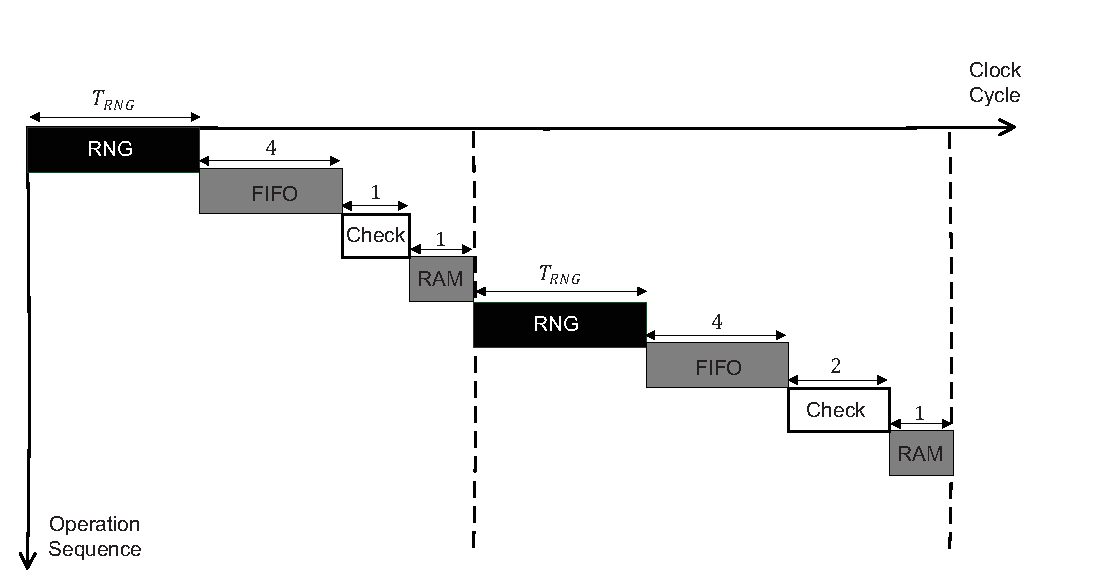
\includegraphics[width=\textwidth]{./fig/pipeline_rng.eps}
\caption{Primitive operation pipelining for Alg.~\ref{alg:prng2}}
\label{fig:pipeline_rng}
\end{subfigure}
\hspace{1em}
\begin{subfigure}[t]{0.45\textwidth}\centering
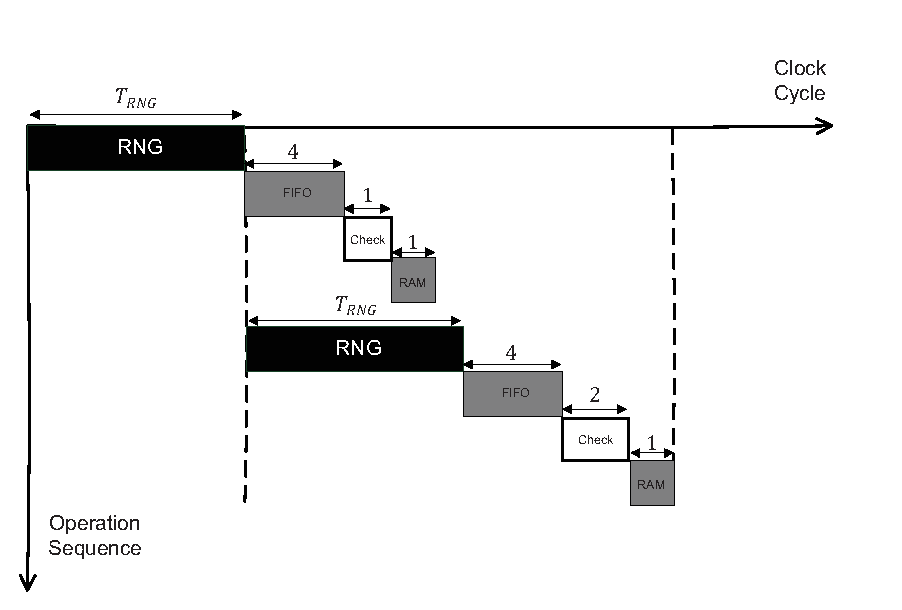
\includegraphics[width=\textwidth]{./fig/pipeline_rng2.eps}
\caption{Optimised operation pipelining for Alg.~\ref{alg:prng2} (initial phase) }
\label{fig:pipeline_rng2}
\end{subfigure}
\begin{subfigure}[t]{0.45\textwidth}\centering
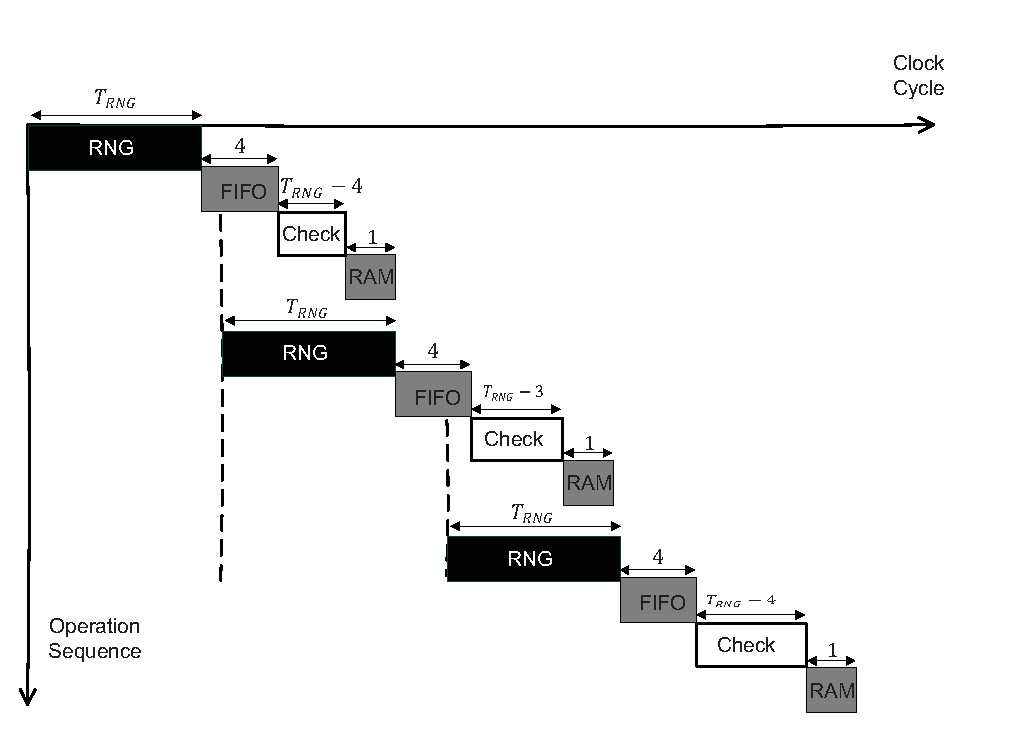
\includegraphics[width=\textwidth]{./fig/pipeline_rng3.eps}
\caption{Optimised operation pipelining for Alg.~\ref{alg:prng2} (final phase) }
\label{fig:pipeline_rng3}
\end{subfigure}
\caption{Timing diagram used for generating a random polynomial with odd weight}
\end{figure*}

\section{Key Generator Architecture}
\begin{figure*}[!tb]
\centering
\begin{subfigure}[t]{0.45\textwidth}\centering
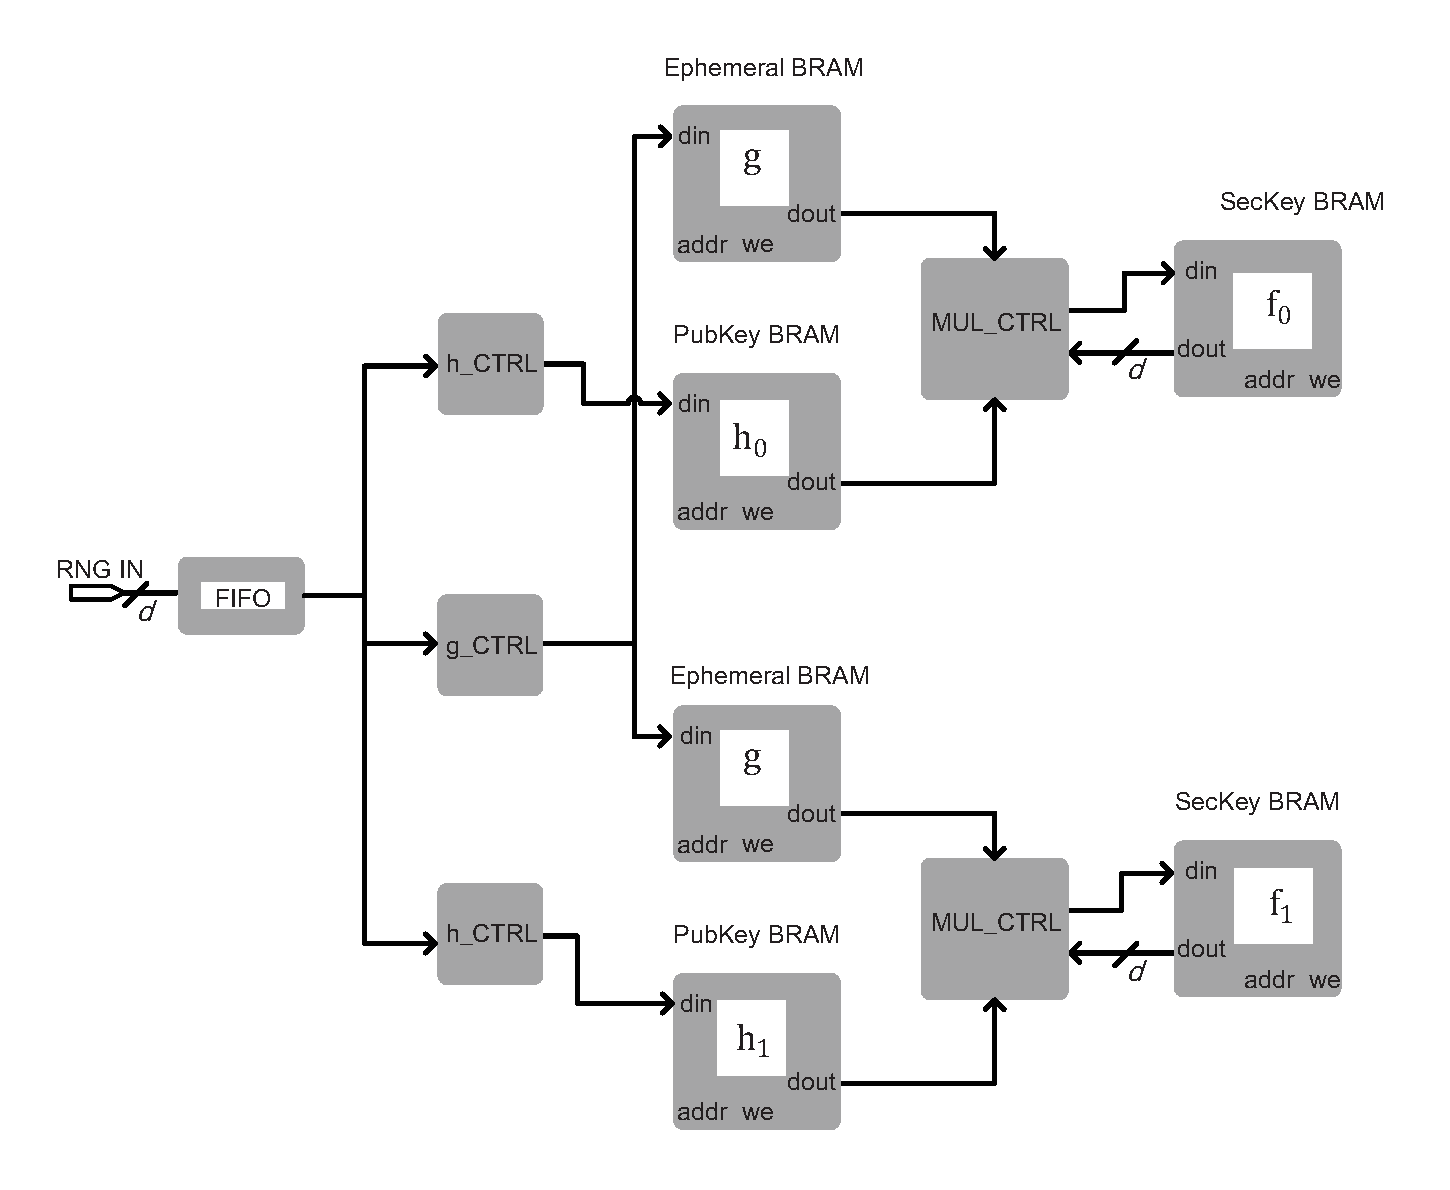
\includegraphics[width=\textwidth]{./fig/BIKE-1.eps}
\caption{BIKE-1}
\label{fig:bike1}
\end{subfigure}
\hspace{1em}
\begin{subfigure}[t]{0.45\textwidth}\centering
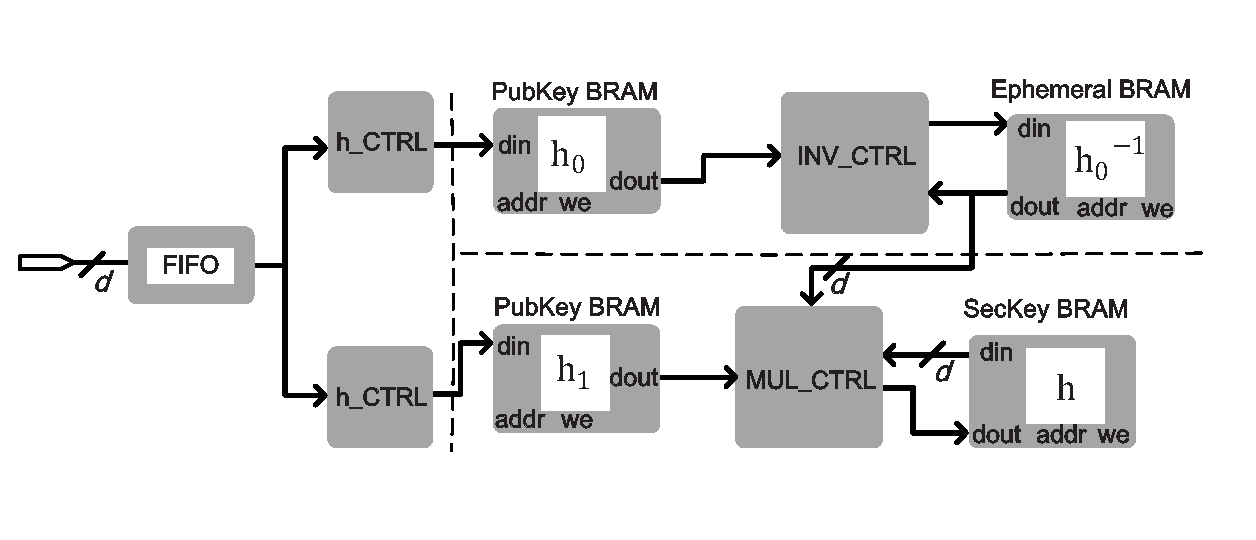
\includegraphics[width=\textwidth]{./fig/BIKE-2.eps}
\caption{BIKE-2 }
\label{fig:bike2}
\end{subfigure}
\begin{subfigure}[t]{0.45\textwidth}\centering
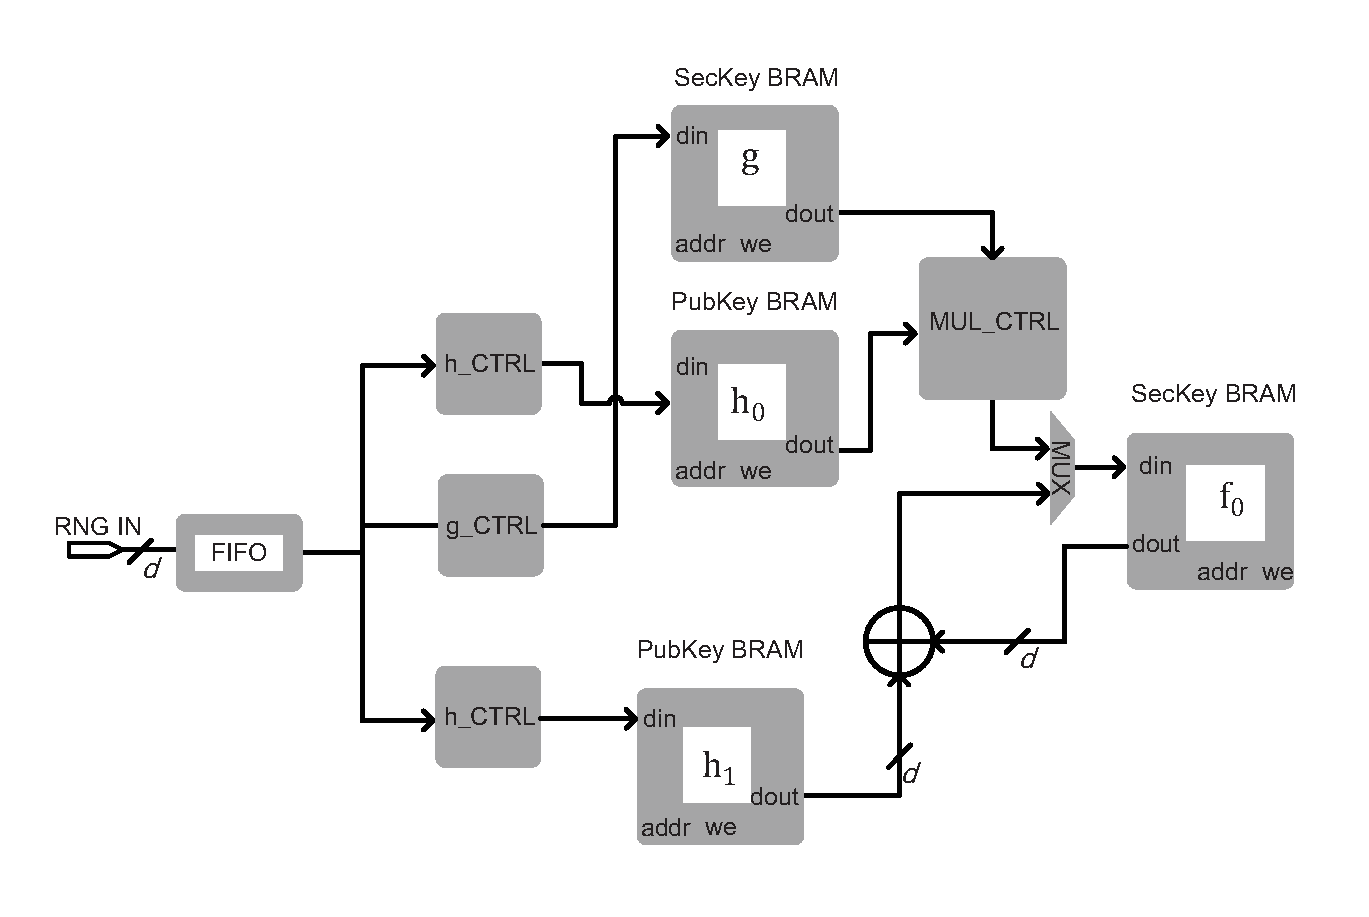
\includegraphics[width=\textwidth]{./fig/BIKE-3.eps}
\caption{BIKE-3 }
\label{fig:bike3}
\end{subfigure}
\caption{Overview of the proposed BIKE architectures}
\end{figure*}

Our key generator performs the computations in BIKE-1/2/3 as shown in Algorithm~\ref{alg:bike1_keygen}, Algorithm~\ref{alg:bike2_keygen}, and Algorithm~\ref{alg:bike3_keygen}. The top level architecture is depicted in Fig.~\ref{fig:bike1}, \ref{fig:bike2}, \ref{fig:bike3}. BIKE-1 and BIKE-2 share a similar architecture where sparse-times-dense multiplication (MUL\_CTRL) is the core functionality. The difference is that BIKE-1 requires two sparse-times-dense multiplications whereas BIKE-3 requires only one sparse-times-dense multiplication plus one addition. In our design, the two multiplications in BIKE-1 are performed simultaneously to improve the timing score and thus the total cycle count of BIKE-1 is close to that of BIKE-3. However, BIKE-3 is the lightest design with the shortest critical path since only one copy of MUL\_CTRL is instantiated here. The module h\_ctrl and g\_ctrl assist to generate the sparse polynomials $h_0,h_1$ and the dense polynomial $g$ as we have discussed in Section 2.6.

BIKE-2 is significantly more computationally intensive than BIKE-1 and BIKE-3 due to the polynomial inversion. The inversion is performed on the module INV\_CTRL as Alg.~\ref{algo:ITA} describes. INV\_CTRL consists of the arithmetic core for continuous square and generic multiplication as illustrated in Section 2.3 and 2.4. After inversion, the dense polynomial $h_0^{-1}$ is obtained and finally the sparse-times-dense multiplication is performed on MUL\_CTRL to extract the secret key $h=h_0^{-1}h_1$.

 The pipeline optimization technique is applied to g\_ctrl, h\_ctrl, MUL\_CTRL, INV\_CTRL for enhancing the timing performance. The detailed schedules have been depicted in Fig. \ref{fig:pipeline_squ2}, ~\ref{fig:pipeline_mul2}, \ref{fig:pipeline_rng3}. As dual-port RAM is instantiated, we are able to load two successive data from secret/public key RAM in one clock cycle to slice registers for fast processing.

\section{Performance Evaluations}
\begin{table*}[!t]\centering
 \caption{Implementation results of BIKE on a Xilinx Virtex-7 XC7V585T FPGA and a Xilinx Spartan-7 XC7S50 FPGA after the place and route process.}
 \label{table:expresult}\centering
 \begin{minipage}{\textwidth}\centering
  \begin{tabular}{lcccccc}
   \hline
   Aspect & \multicolumn{2}{c}{BIKE-1 KeyGen} & \multicolumn{2}{c}{BIKE-2 KeyGen} & \multicolumn{2}{c}{BIKE-3 KeyGen}\\
    & Virtex-7 & Spartan-7  & Virtex-7 & Spartan-7  & Virtex-7 & Spartan-7\\
   \hline
   FFs &1055   &993  &2159 &2098 &955 &911\\
   LUTs & 1970  &1897  &4445 &3872&1482&1402  \\
   Slices& 612 &544  &1483 &1272&472&423  \\
   BRAM & 7  &7  &10 & 10& 4&4\\
   \hline
   Frequency &  350 MHz  & 160 MHz &320 MHz & 150 MHz  & 360 MHz & 200 MHz\\
   Time/Op &  0.273 $ms$ &  0.597 $ms$ & 6.719 $ms$& 14.334 $ms$ &0.273 $ms$  & 0.492 $ms$\\
   \hline
   Compute $h_0$ & \multicolumn{2}{c}{$1279$ cycles} & \multicolumn{2}{c}{$1279$ cycles}  & \multicolumn{2}{c}{$1062$ cycles}\\
   Compute $h_1$& \multicolumn{2}{c}{$1279$ cycles} & \multicolumn{2}{c}{$1279$ cycles} & \multicolumn{2}{c}{$1062$ cycles}\\
   Compute $g$ & \multicolumn{2}{c}{$2068$ cycles} & \multicolumn{2}{c}{---} & \multicolumn{2}{c}{$2250$ cycles}\\
   Compute ${h_0}^{-1}$ & \multicolumn{2}{c}{---} & \multicolumn{2}{c}{$2,056,683$ cycles} &\multicolumn{2}{c}{---}\\
   Compute $f_0$ & \multicolumn{2}{c}{$90,880$ cycles} & \multicolumn{2}{c}{---} &\multicolumn{2}{c}{$94,135$ cycles}\\
   Compute $f_1$ & \multicolumn{2}{c}{$90,880$ cycles}  & \multicolumn{2}{c}{---} &\multicolumn{2}{c}{---}\\
   Compute $h$  &  \multicolumn{2}{c}{---}          & \multicolumn{2}{c}{$90,880$ cycles} & \multicolumn{2}{c}{---}\\
   \hline
   Overall & \multicolumn{2}{c}{$95,506$ cycles} & \multicolumn{2}{c}{$2,150,121$ cycles} & \multicolumn{2}{c}{$98,509$ cycles}\\
   \hline
  \end{tabular}
  \end{minipage}
\end{table*}



In this section, we present our BIKE implementation results in FPGA. All the results are obtained post place-and-route for a  Xilinx high-end FPGA device --- Virtex XC7V585T  and a low-end FPGA device ---  Spartan XC7S50 FPGA using Xilinx Vivado v2018.1 which demonstrate the compactness of our design on both platforms. To the best of our knowledge, this work is the first one that reports the performance results of BIKE key generation on an FPGA platform. As shown in Table~\ref{table:expresult}, our BIKE-1 key generator on the Virtex-7 device runs at 350~MHz and generates one key pair  in $95,506$ cycles, that is 0.273 $ms$ of operation time. It runs on the Spartan-7 device at 160~MHz and generates one key pair in 0.597~$ms$. The area footprint is low (612 slices and 544 slices on Virtex-7 and Spartan-7 respectively) as our proposed architecture executes all operations  in digit level (here in this concrete experiment, 64-bits of data are operated per time), which costs limited hardware resources. Our BIKE-3 key generator performs even better: It runs faster in $0.273$ $ms$ and $0.492$ $ms$ on Virtex-7 and Spartan-7, respectively. The slice overheads are also lower as BIKE-3 carries one copy of the core unit, sparse-times-dense multiplication whereas BIKE-1 has two of them. The cycle count is slightly worse than that of BIKE-1 as BIKE-3 requires an extra polynomial addition to compute the secret key $f_0$.

On the other hand, our BIKE-2 key generator runs at 320 MHz and 150 MHz on the Virtex-7 and Spartan-7 device respectively, and generates a key pair in $2,150,121$ cycles. This cycle count is equivalent to $6.719$ ms and $14.334$ ms of operating time for Virtex-7 and Spartan-7, respectively. It is noteworthy to mention that BIKE-2 timing performance is  two orders of magnitude worse than BIKE-1 and BIKE-3.  Such performance gap is due to the costly polynomial inversion in BIKE-2. Nevertheless, by using the proposed generic multiplication algorithm and continuous square algorithm, the BIKE-2 timing is significantly improved and preserves the constant-time execution. The slice usage is also conservative, increasing by 2-3 times compared with BIKE-1 and BIKE-2.  The memory overhead is larger than that of BIKE-1/2 since inversion requests to save some ephemeral variables.

In the following, we compare our work with state-of-arts software implementations on either CPUs or micro-controllers. It is worth noting that comparison of our results with other software implementations is not fair since the platform used differs significantly. We attempt to compare the performance in the metric of cycle counts which is an platform independent indicator, given in Table \ref{table:compare}.
First, we compare with the standard BIKE specification implementation \cite{aragon2017bike} which is also submitted for NIST PQC standardization. The experiments from \cite{von2014lightweight} is equipped with an Intel i5 CPU running at 1.8 GHz and 32 GB RAM, 32K L1d and L1i cache, 256K L2 cache, and 4096K L3 cache. Their implementation is non-constant time and is much slower than ours. The micro-controller implementation from \cite{maurich2015implementing} is performed on ARM Cortex-M4 and uses obsolete BIKE-2 system parameters with 80-bit security level which is not recommended in the NIST PQC standardization. Despite the insufficiently 80-bit SL parameters used in \cite{maurich2015implementing}, their implementation is non-constant time and costs huge cycle counts (148.5 million).  An optimized software implementation for BIKE is reported in \cite{drucker2017toolbox}. This additional implementation is equipped with an Intel i5 CPU running at 3.0 GHz and 70 GB RAM, 32K L1d and L1i cache, 1024K L2 cache, and 25,344K L3 cache. The core functionality is written in x86 assembly, and wrapped by assisting C code.
The implementation uses the PCLMULQDQ architecture extension to enable carry-less multiplication for performance gain. Despite these dedicate and platform-dependent optimizations, our results are comparable and even better than \cite{drucker2017toolbox}. The performance gain of our design comes from two aspects: first, the pipelining parallelization is proposed for core functions including squaring, multiplication. second, the proposed continuous squaring, generic multiplication, and sparse-times-dense multiplication has lower communication overheads to external memory which facilitate computational accelerations on FPGA.

\begin{table*}[!t]\centering
\caption{Performance comparison of our FPGA implementation with dedicate software implementations.}
\label{table:compare}
\begin{minipage}{\textwidth}\centering
\scalebox{1.0}{\begin{tabular}{lcccc}
\hline
Scheme &{SL [bit]}&  Implementation & Platform & \tabincell{c}{Performance\\{} [in millions of cycles]}\\
\hline
\multirow{3}{*}{\textbf{BIKE-1}} & 128 & Ours, constant-time & FPGA & 0.095\\
                                & 128 & \cite{aragon2017bike} & CPU & $\approx 0.73$\\
                                & 128 & \cite{drucker2017toolbox} & CPU & 0.09\\
\hline
\multirow{4}{*}{\textbf{BIKE-2}} & 128 & Ours, constant-time & FPGA & 2.15\\
                                & 128 & \cite{aragon2017bike} & CPU &$\approx 6.3$\\
                                & 128 & \cite{drucker2017toolbox}& CPU & 4.38\\
                                 & 80 & \cite{maurich2015implementing} & Micro-controller &$\approx 148.5$\\
\hline
\multirow{2}{*}{\textbf{BIKE-3}} & 128 & Ours, constant-time & FPGA & 0.098\\
                                 & 128 & \cite{aragon2017bike} & CPU &$\approx 0.43$ \\
\hline
\end{tabular}}
\end{minipage}
\end{table*}


\begin{table*}[!t]\centering
\caption{Performance comparison of our FPGA implementation with other code-based key generators.}
\label{table:compare}
\begin{minipage}{\textwidth}\centering
\scalebox{0.9}{\begin{tabular}{lcccccccc}
\hline
Scheme &\tabincell{c}{SL\\{} [bit]}&Platform &$f$[MHz] & Time/Op & Cycles  & Slices & BRAM\\
\hline
MDPC code:\\
\textbf{Ours (BIKE-1)} & \multirow{3}{*}{\textbf{128}} & \multirow{3}{*}{Virtex-7} & {\textbf{350}}  & $\mathbf{0.273 ms}$& $9.55\times 10^4$  & \textbf{612} & \textbf{7}\\
\textbf{Ours (BIKE-2)} &  &  & {\textbf{320}}  & $\mathbf{6.719 ms}$& $2.15\times 10^6$  & \textbf{1483} & \textbf{10}\\
\textbf{Ours (BIKE-3)} &  &  & {\textbf{360}}  & $\mathbf{0.273 ms}$& $9.85\times 10^4$  & \textbf{472} & \textbf{4}\\
\hline
Goppa code:\\
\cite{wang2018fpga} &{256} &{Virtex Ultrascale+} & {225}   & $3.98ms$    & $\approx 1.01\times 10^{11}$  & {112,845}& {375}\\
\cite{wang2018fpga} &{103} &{Virtex 5} & {168}   & $16 ms$    & $\approx 2.72\times 10^6$  & {8171}& {89}\\
\cite{shoufan2010novel} &{103} &{Virtex 5} & {163}   & $90 ms$    & $\approx 1.47\times 10^7$  & {17,280}& {148}\\
\hline
\end{tabular}}
\end{minipage}
\end{table*}

Second, we compare our work with other existing hardware solutions based on Goppa codes \cite{wang2018fpga,shoufan2010novel}. As the state-of-art reference we consider the implementation reported in \cite{wang2018fpga}, where scalability is tested with different system parameters and FPGA platforms. We extract from \cite{wang2018fpga} the experimental results at 256-bit SL and 103-bit SL on Xilinx FPGAs to provide direct and fair comparison.
It is seen that for almost the same security level, Goppa codes require much more memory and computation time to generate the public/secret key. Such memory overhead is inevitable in Goppa code schemes as Goppa code cannot benefit from quasi-cyclic construction to compress the key size.
Conversely, our work based on quasi-cyclic codes is identified as a scalable lightweight design which shares high-speed and low-storage characteristics.

\section{Conclusions}
This paper presented a lightweight yet fast hardware-based key generator of a key encapsulation mechanism based on MDPC, called BIKE, both of which are second-round candidates for the NIST PQC competition. Novel multiplication and squaring algorithms were proposed to accelerate the key generation with low logic overhead. This work also presented optimized pipeline scheduling for fast execution of the core functions. The methods above are generic and applicable to other code-based schemes if the underlying code is quasi-cyclic.

%
% ---- Bibliography ----
%
% BibTeX users should specify bibliography style 'splncs04'.
% References will then be sorted and formatted in the correct style.
%
% \bibliographystyle{splncs04}
% \bibliography{mybibliography}
%
\bibliographystyle{abbrv}
\bibliography{./reference}

\end{document}
